\documentclass[12pt,a4paper]{article}

\usepackage{float}
\usepackage{subcaption}

% Idioma e acentuação
\usepackage[brazil]{babel}
\usepackage[T1]{fontenc}
\usepackage[utf8]{inputenc}
\usepackage{url}
% Fonte
\usepackage{mathptmx}

% Margens ABNT
\usepackage[
  left=3cm,
  right=2cm,
  top=3cm,
  bottom=2cm
]{geometry}

% Espaçamento
\usepackage{setspace}
\usepackage{parskip}
\onehalfspacing % 1,5

% Parágrafo
\usepackage{indentfirst}
\setlength{\parindent}{1.25cm}

% Cabeçalho (numeração no topo)
\usepackage{fancyhdr}
\setlength{\headheight}{15pt}
\pagestyle{fancy}
\fancyhf{}
\fancyhead[R]{\thepage}
\renewcommand{\headrulewidth}{0pt}

% Sumário
\usepackage{tocloft}
\renewcommand{\contentsname}{SUMÁRIO}
\renewcommand{\cftdotsep}{1}

\usepackage[num]{abntex2cite}
\usepackage{longtable}
\usepackage{array}
\usepackage[table]{xcolor}

% Gráficos
\usepackage{graphicx}


\newcommand{\ucitem}[2]{\par\noindent\hangindent=1.6em\hangafter=1\makebox[1.6em][l]{#1}#2}
\newcommand{\ucsubitem}[2]{\par\noindent\hangindent=3.2em\hangafter=1\hspace*{1.6em}\makebox[1.6em][l]{#1}#2}
\newcommand{\pkg}[1]{{\ttfamily\hyphenchar\font=`\-\relax #1}}




\begin{document}





% ---------- CAPA ----------
\begin{titlepage}
\centering

{\small
Universidade Federal Fluminense -- UFF\\
Campus Universitário de Rio das Ostras\\
Instituto de Ciência e Tecnologia
}

\vspace{8cm}


{\bfseries
\MakeUppercase{Talkie: Plataforma Web Voltada ao Registro e Comunicação}
}

\vspace{8cm}

{\normalsize
Isabelle Pires Vimercati
}

\vfill

Rio das Ostras\\
2025

\end{titlepage}

\clearpage
% ---------- FIM DA CAPA ----------



% -------- PÁGINAS PRÉ-TEXTUAIS (sem numeração visível)
\pagenumbering{gobble}

\clearpage

\begin{center}
\textbf{\Large Resumo}
\end{center}

\addcontentsline{toc}{section}{Resumo}

Os cidadãos brasileiros, em suas rotinas diárias, enfrentam diversos problemas
cotidianos que, a depender de seu contexto social e urbano, podem apresentar
naturezas distintas. Entretanto, observa-se que há dificuldades burocráticas e
operacionais no registro de denúncias e ocorrências junto aos órgãos responsáveis,
o que pode comprometer a resolução desses problemas e impactar negativamente a
vivência em sociedade. Diante disso, este trabalho propõe o desenvolvimento de um
sistema Web com o objetivo de auxiliar o registro e o encaminhamento de ocorrências
identificadas pelos cidadãos aos órgãos competentes. A proposta consiste em utilizar
a tecnologia como ferramenta para facilitar a comunicação entre a população e as
instituições e contribuir para o bem-estar social.

\clearpage

\begin{center}
\textbf{\Large Abstract}
\end{center}

\addcontentsline{toc}{section}{Abstract}

In their daily lives, Brazilian citizens face a variety of everyday problems that, depending on their social and urban context, may differ in nature. However, bureaucratic and operational challenges in reporting incidents and complaints to the appropriate public authorities are commonly observed, which may hinder the resolution of these issues and negatively impact social well-being. 
This study proposes the development of a web-based system designed to support the registration and forwarding of incidents identified by citizens to the responsible public agencies. The proposed solution uses technology as a tool to facilitate communication between the population and public institutions, thereby contributing to improved public services and social well-being. 

\clearpage

\clearpage
\listoffigures
\clearpage

\section*{Lista de Siglas}
\addcontentsline{toc}{section}{Lista de Siglas}

\begin{description}
    \item[API] Application Programming Interface
    \item[CPF] Cadastro de Pessoas Físicas
    \item[CSS] Cascading Style Sheets
    \item[DTO] Data Transfer Object
    \item[FA] Fluxo Alternativo
    \item[FE] Fluxo de Exceção
    \item[HTML] HyperText Markup Language
    \item[HTTP] HyperText Transfer Protocol
    \item[HTTPS] HyperText Transfer Protocol Secure
    \item[IA] Inteligência Artificial
    \item[JPA] Jakarta Persistence
    \item[JPEG] Joint Photographic Experts Group
    \item[JSON] JavaScript Object Notation
    \item[JWT] JSON Web Token
    \item[MCP] Model Context Protocol
    \item[PNG] Portable Network Graphics
    \item[REST] Representational State Transfer
    \item[RF] Requisito Funcional
    \item[RNF] Requisito Não Funcional
    \item[SQL] Structured Query Language
    \item[UC] Caso de Uso (\textit{Use Case})
    \item[UML] Unified Modeling Language
\end{description}
\clearpage

\tableofcontents
\clearpage

% -------- TEXTO (numeração começa aqui)
\pagenumbering{arabic}
\setcounter{page}{4} 

\section{Introdução}
\subsection{Motivação}
O avanço das tecnologias da informação e sua crescente integração ao cotidiano da sociedade têm transformado significativamente a forma como os usuários interagem com serviços e instituições. Entre os impactos positivos desse processo, destaca-se a modernização dos serviços oferecidos à população, proporcionando maior agilidade, acessibilidade e eficiência em diversas atividades. Entretanto, muitos processos ainda dependem de procedimentos burocráticos e de canais de comunicação pouco acessíveis, dificultando o registro de demandas e o encaminhamento de ocorrências aos responsáveis por sua resolução.

Nesse contexto, observa-se que diferentes setores podem ser beneficiados pela adoção de sistemas destinados ao registro e gerenciamento de ocorrências, contribuindo para a melhoria da qualidade de vida e da eficiência operacional de seus usuários. No ambiente universitário, por exemplo, estudantes poderiam registrar de forma simples problemas relacionados à infraestrutura, manutenção ou serviços, encaminhando essas informações diretamente aos setores competentes. Além de facilitar a comunicação entre a comunidade acadêmica e a instituição, tal solução promoveria maior transparência no tratamento das demandas apresentadas.

Outro cenário de aplicação corresponde ao ambiente industrial, como plataformas de petróleo, especialmente nas atividades de manutenção. Nesses locais, um sistema de registro de ocorrências pode contribuir para a identificação e o acompanhamento de problemas estruturais e operacionais, auxiliando no planejamento de manutenções preventivas e corretivas. Dessa forma, o registro centralizado das ocorrências favorece uma resposta mais rápida às demandas e contribui para a melhoria dos processos de manutenção e da segurança operacional.

Diante desse cenário, a escolha deste tema fundamenta-se na proposta de desenvolvimento de uma ferramenta capaz de se adaptar a diferentes contextos de utilização, de acordo com as necessidades específicas de cada ambiente. Ao oferecer uma solução flexível para o registro, o gerenciamento e o encaminhamento de ocorrências, busca-se estabelecer um mecanismo que possa ser aplicado em distintos setores, promovendo uma comunicação mais eficiente entre os usuários e os responsáveis pela resolução das demandas, além de contribuir para a otimização dos processos envolvidos.

\subsection{Objetivos}
O objetivo geral deste trabalho consiste no desenvolvimento de um sistema web destinado ao registro, ao gerenciamento e ao encaminhamento de ocorrências, permitindo centralizar as demandas registradas pelos usuários e direcioná-las aos responsáveis por sua resolução. Além disso, busca-se proporcionar maior transparência no acompanhamento do ciclo de vida das ocorrências, desde seu registro até a apresentação de seu status e de sua resolução.

Como característica central da solução, pretende-se desenvolver uma plataforma flexível e personalizável, capaz de adaptar as categorias de ocorrências e os fluxos de encaminhamento às necessidades específicas de diferentes ambientes de aplicação. Dessa forma, busca-se oferecer uma interface intuitiva e acessível a usuários com diferentes níveis de familiaridade com tecnologias digitais, contribuindo para a redução de barreiras no registro de demandas e para o aprimoramento da comunicação entre os usuários e as instituições ou equipes responsáveis por seu atendimento.
\clearpage

\section{Trabalhos Relacionados}
Nesta seção será abordada a análise de soluções e projetos semelhantes ao proposto, permitindo a identificação de abordagens existentes e contribuições relevantes para o desenvolvimento. Serão apresentados três trabalhos de aplicações que contém as funcionalidades de registro de ocorrências para auxiliar a contextualização do leitor. \\

Diversas aplicações têm sido desenvolvidas para auxiliar usuários por meio de registros e compartilhamento de ocorrências em ambientes urbanos, contribuindo para a melhoria da mobilidade, segurança e gestão pública. Dentre as aplicações estão o Waze\cite{waze}, COR.Rio\cite{cor-rio} e Rio1746\cite{1746}, destaques por possuírem funcionalidades semelhantes ao do trabalho proposto.

O Waze é uma aplicação de navegação colaborativa amplamente utilizada ao redor do mundo, cujo diferencial está na participação ativa dos usuários no registro de ocorrências em tempo real. O aplicativo permite que os usuários informem diferentes tipos de eventos, como acidentes, congestionamentos, vias interditadas, obras, radares, veículos parados e perigos na pista. A Figura~\ref{fig:waze-conjunto} apresenta as principais funcionalidades de
registro de ocorrências do aplicativo Waze.


\begin{figure}[H]
    \centering

    \begin{subfigure}{0.3\linewidth}
        \centering
        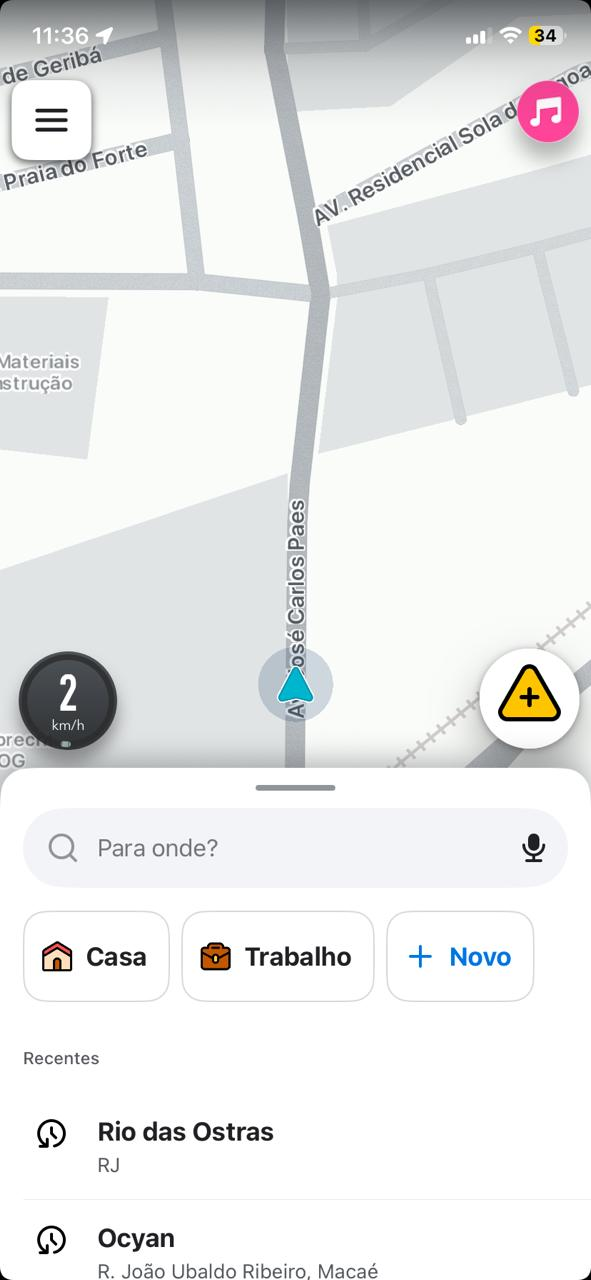
\includegraphics[width=\linewidth]{imagens/WhatsApp Image 2025-12-18 at 19.08.00.jpeg}
        \caption{Visualização do mapa}
        \label{fig:waze-a}
    \end{subfigure}
    \hfill
    \begin{subfigure}{0.3\linewidth}
        \centering
        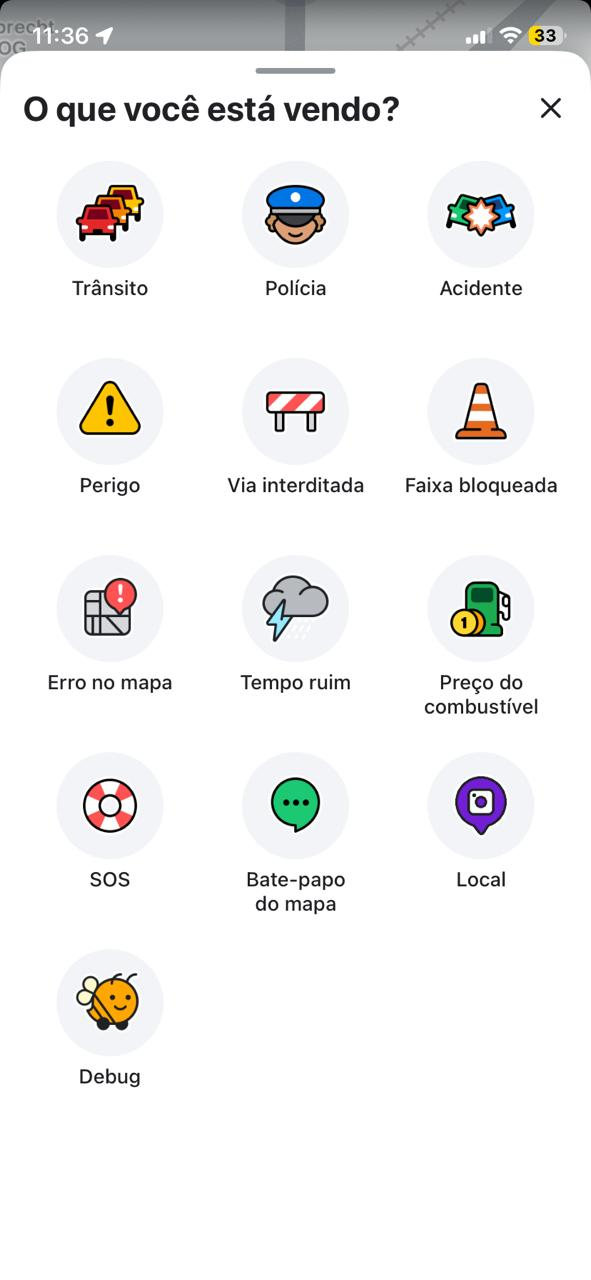
\includegraphics[width=\linewidth]{imagens/WhatsApp Image 2025-12-18 at 19.08.00 (1).jpeg}
        \caption{Tipos de ocorrências}
        \label{fig:waze-b}
    \end{subfigure}
    \hfill
    \begin{subfigure}{0.3\linewidth}
        \centering
        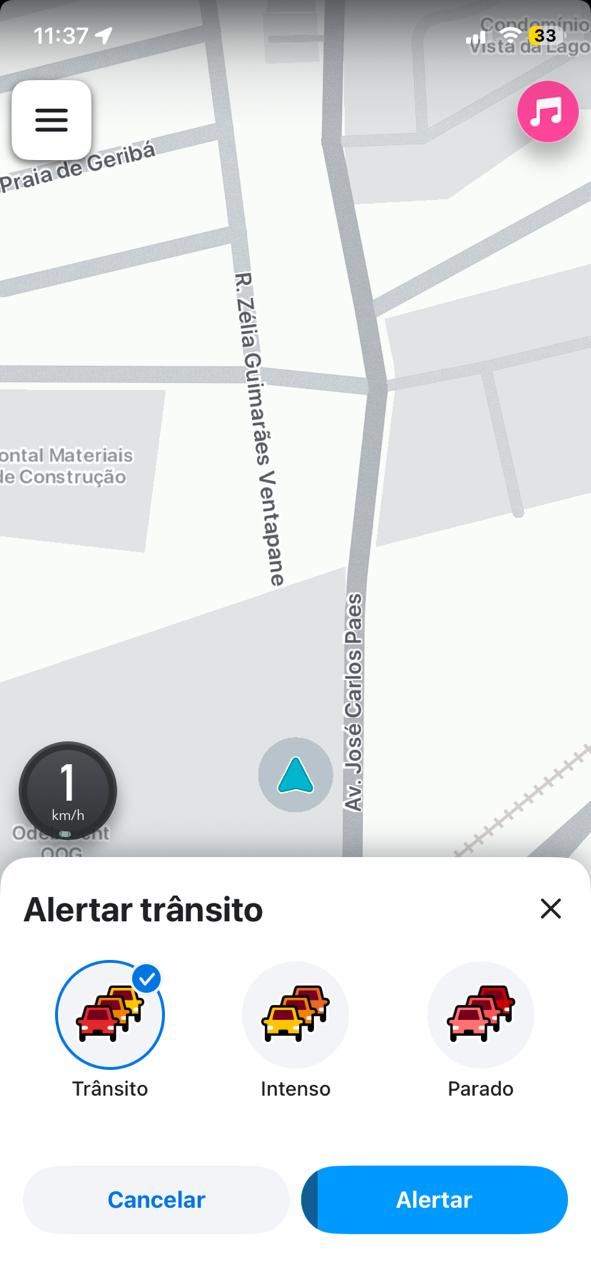
\includegraphics[width=\linewidth]{imagens/WhatsApp Image 2025-12-18 at 19.08.00 .jpeg}
        \caption{Subtipos de ocorrências}
        \label{fig:waze-c}
    \end{subfigure}

    \caption{Funcionalidades do aplicativo Waze}
    \vspace{0.2cm}
    \small Fonte: aplicativo Waze (2025).
    \label{fig:waze-conjunto}
\end{figure}


Essa variedade de categorias permite uma visão mais ampla dos caminhos, possibilitando o usuário a tomar decisões sobre possíveis rotas alternativas. Além disso, as informações compartilhadas impactam diretamente no cálculo de rotas do aplicativo, tornando-o dinâmico e responsivo às condições reportadas. No entanto, seu escopo foca em eventos relacionados ao trânsito e não há uma abrangência em outros tipos de ocorrências de interesse geral da população.

Outro trabalho de destaque é o aplicativo COR.Rio, desenvolvido pelo Centro de Operações do Rio, que tem como objetivo informar eventos que impactem a rotina da cidade do Rio de Janeiro. O aplicativo permite uma comunicação um pouco mais ampla do que o Waze, informando sobre trânsito, condições climáticas, acidentes, interdições, grandes eventos e situações de emergência. 

\begin{figure}[H]
    \centering

    \begin{subfigure}{0.3\linewidth}
        \centering
        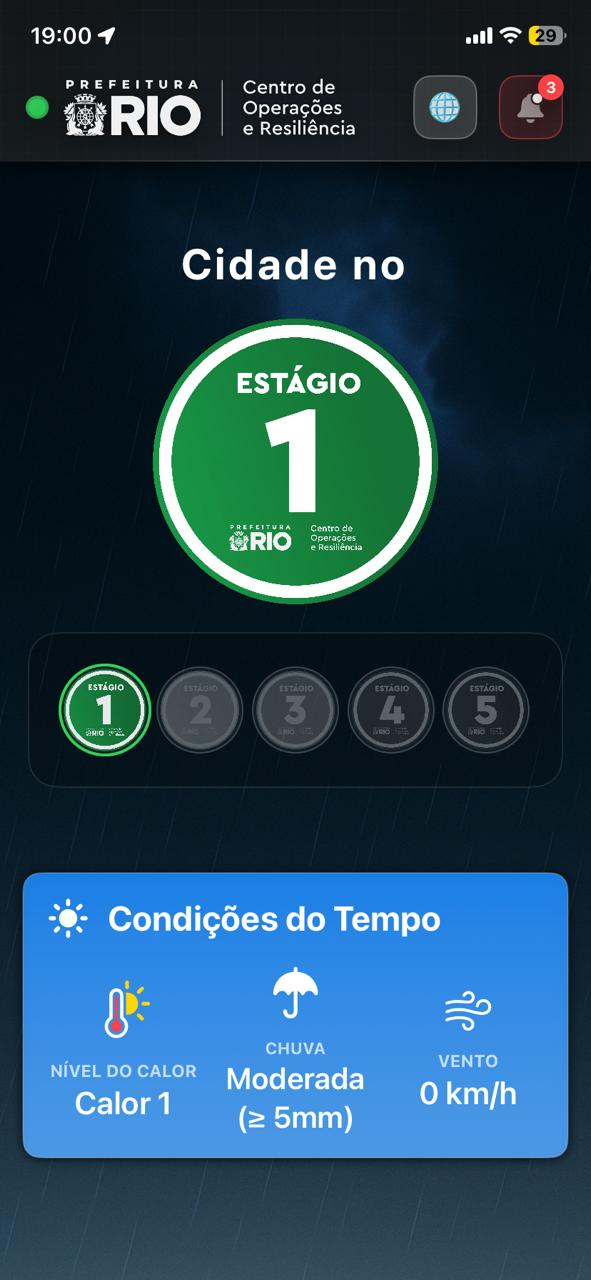
\includegraphics[width=\linewidth]{imagens/COR1.jpeg}
        \caption{Tela inicial do app}
        \label{fig:COR-a}
    \end{subfigure}
    \hfill
    \begin{subfigure}{0.3\linewidth}
        \centering
        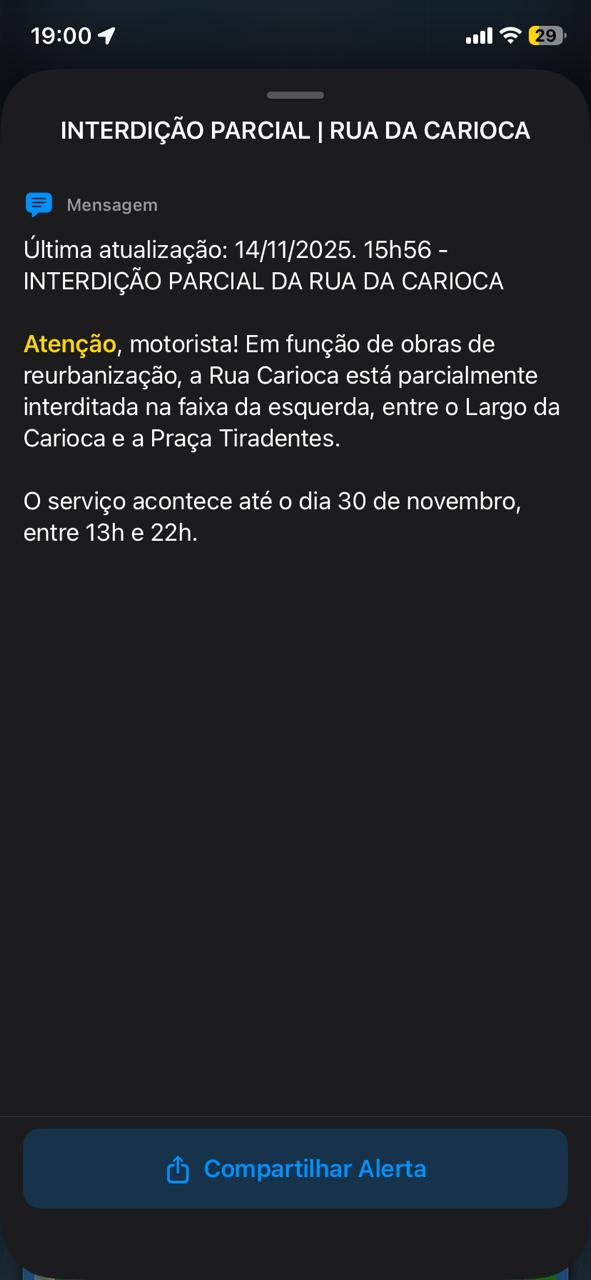
\includegraphics[width=\linewidth]{imagens/COR2.jpeg}
        \caption{Ocorrência registrada}
        \label{fig:COR-b}
    \end{subfigure}
    \hfill
    \begin{subfigure}{0.3\linewidth}
        \centering
        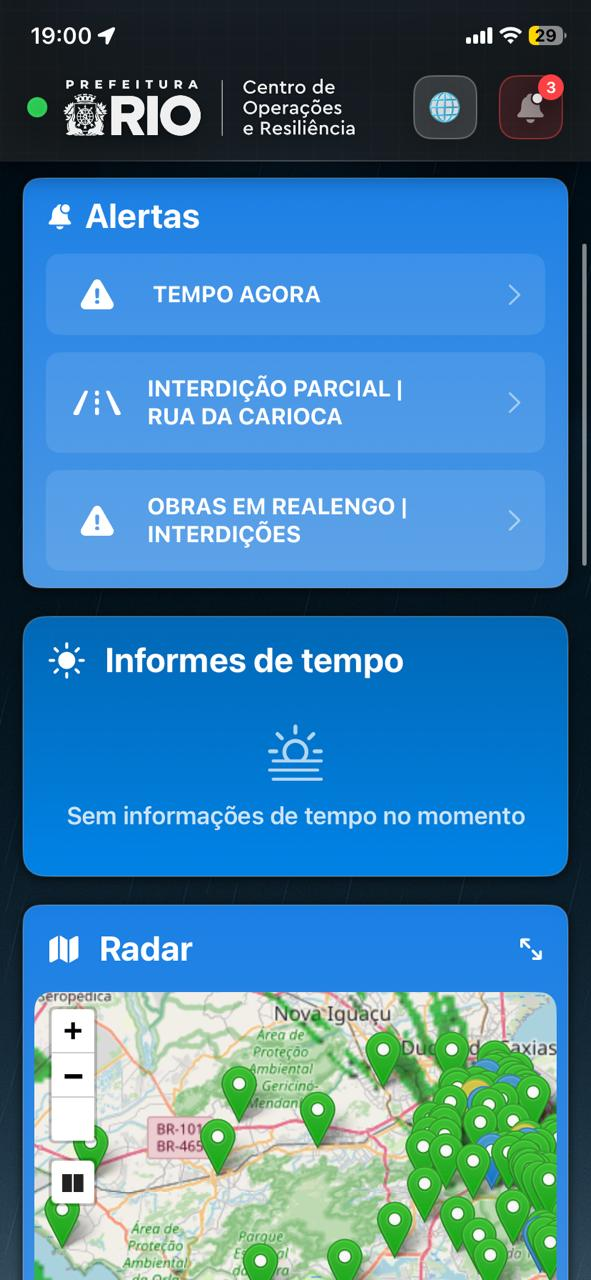
\includegraphics[width=\linewidth]{imagens/COR3.jpeg}
        \caption{Aletas criados}
        \label{fig:COR-c}
    \end{subfigure}

    \caption{Funcionalidades do aplicativo COR.Rio}
    \vspace{0.2cm}
    \small Fonte: Aplicativo COR.Rio (2025).
    \label{fig:cor-conjunto}
\end{figure}


Diferente do Waze, o COR.Rio centraliza as informações provenientes de órgãos oficiais, o que agrega maior confiabilidade às informações. Entretanto, a participação direta do cidadão no registro de ocorrência é limitada, uma vez que o aplicativo atua mais como um canal institucional.

Outro trabalho relevante é o Rio1746, uma plataforma oficial da Prefeitura do Rio de Janeiro voltada para o suporte ao cidadão. O sistema permite que os usuários se cadastrem e registrem solicitações, reclamações, denúncias e ocorrências relacionadas a diversos serviços públicos, como iluminação, limpeza urbana, conservação de vias e ordem pública. O Rio1746 se detaca não somente pela ampla variedade de tipos de ocorrências, mas pela sua funcionalidade de acompanhar o andamento das solicitações. No entanto, seu foco é voltado ao atendimento administrativo, não oferecendo a visualização em tempo real ou compartilhamento das ocorrências.

\begin{figure}[H]
    \centering

    \begin{subfigure}{0.3\linewidth}
        \centering
        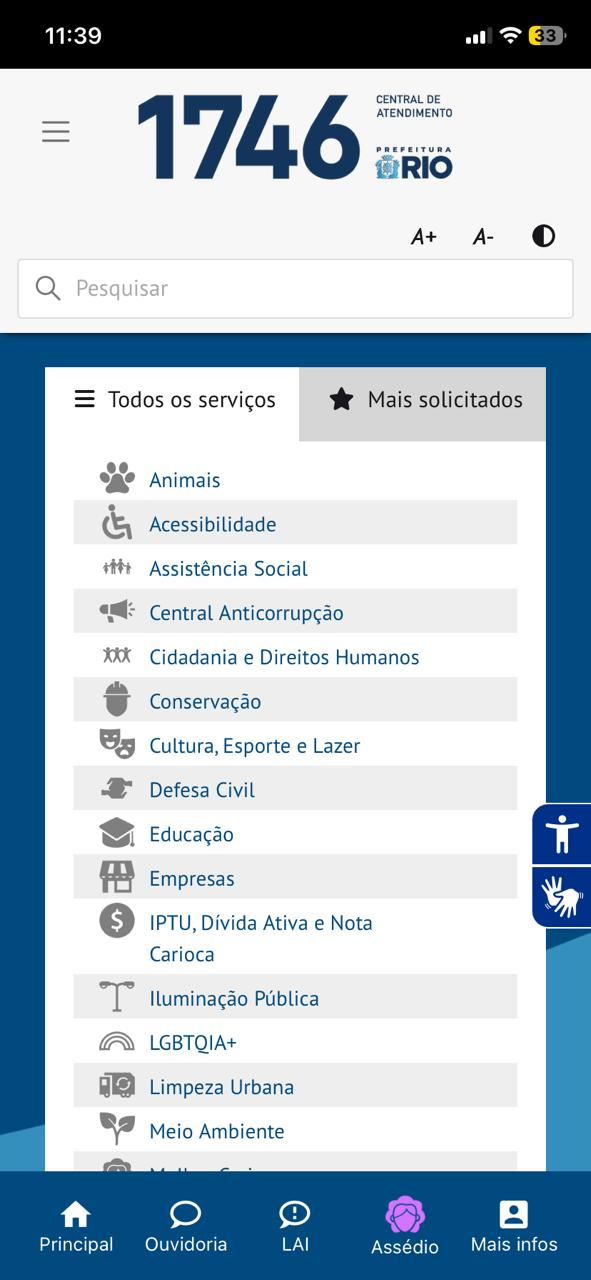
\includegraphics[width=\linewidth]{imagens/Rio1746.jpeg}
        \caption{Tela inicial do app}
        \label{fig:rio-a}
    \end{subfigure}
    \hfill
    \begin{subfigure}{0.3\linewidth}
        \centering
        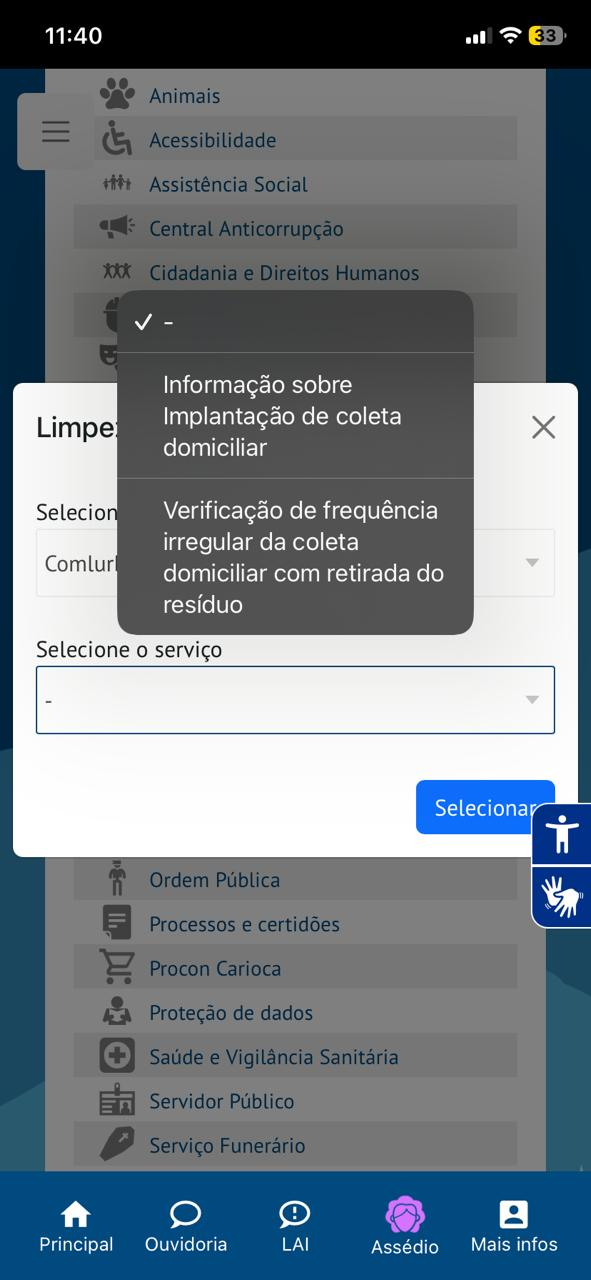
\includegraphics[width=\linewidth]{imagens/Rio17462.jpeg}
        \caption{Menu de solicitações}
        \label{fig:rio-b}
    \end{subfigure}
    \hfill
    \begin{subfigure}{0.3\linewidth}
        \centering
        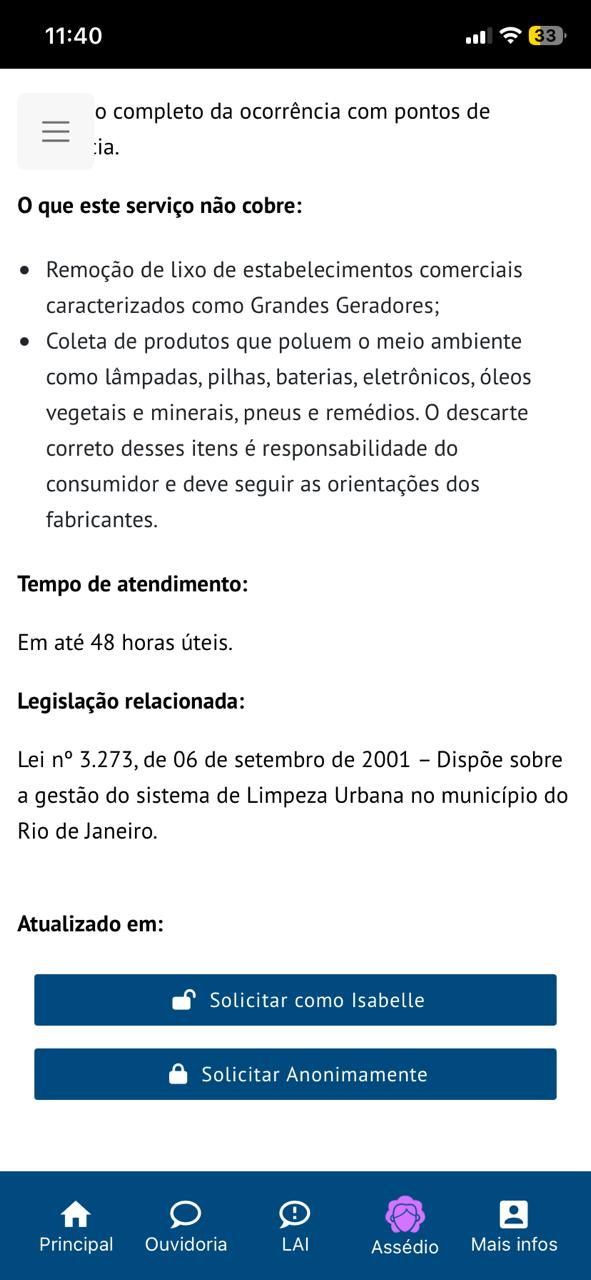
\includegraphics[width=\linewidth]{imagens/Rio17463.jpeg}
        \caption{Informações da solicitação}
        \label{fig:rio-c}
    \end{subfigure}

    \caption{Funcionalidades do aplicativo Rio1746}
    \vspace{0.2cm}
    \small Fonte: Aplicativo Rio1746 (2025).
    \label{fig:rio-conjunto}
\end{figure}

A análise desses trabalhos evidencia diferentes abordagens para o registro e disseminação de ocorrências. Enquanto o Waze se destaca pela colaboração dos usuários e pela diversidade, o COR.Rio prioriza a divulgação de dados confiáveis em tempo real, e o Rio1746 foca no suporte ao cidadão após o registro. O sistema proposto busca extrair aspectos positivos de ambas as soluções, como categorização das ocorrências, a participação do usuário e a centralização das informações.
\clearpage

\section{Proposta do Sistema}
Nesta seção, será abordada a proposta do sistema desenvolvido, através dos requisitos, funcionais e não funcionais, diagramas de caso de uso e modelagem lógica. 

\subsection{Requisitos}
A engenharia de requisitos é o processo responsável por descobrir, analisar,
documentar e validar os serviços que um sistema deve oferecer e as restrições
sob as quais ele deve operar \cite{sommerville}. Nesse contexto, um requisito
pode ser entendido como uma condição ou capacidade necessária para que o
usuário resolva um problema ou alcance um objetivo, ou ainda como aquilo que
o sistema deve atender para satisfazer um contrato, padrão, especificação ou
outro documento formalmente imposto.

\subsubsection{Requisitos Funcionais}
Os requisitos funcionais descreve as ações, funcionalidades, comportamentos e capacidades complexas que um software deve executar, de acordo com cada situação.
Na Tabela~\ref{tab:requisitos-funcionais}, serão apresentados os requisitos funcionais do trabalho em questão. Os requisitos são apresentados com identificador, sua descrição e sua classificação de prioridade.

\begin{longtable}{|p{0.10\textwidth}|p{0.66\textwidth}|p{0.14\textwidth}|}
\caption{Requisitos funcionais}
\label{tab:requisitos-funcionais} \\
\hline
\textbf{ID} & \textbf{Descrição} & \textbf{Prioridade} \\
\hline
\endfirsthead

\hline
\textbf{ID} & \textbf{Descrição} & \textbf{Prioridade} \\
\hline
\endhead

\hline
\endfoot
\rowcolor{gray!20}
\multicolumn{3}{|c|}{\textbf{Cadastro e Acessos}} \\
\hline
RF01 & O sistema deve permitir que um visitante crie uma conta & ALTA \\
\hline
RF02 & O sistema deve permitir que um usuário cadastrado acesse a plataforma & ALTA \\
\hline
RF03 & O sistema deve permitir que um usuário autenticado encerre sua sessão & MÉDIA \\
\hline
\rowcolor{gray!20}
\multicolumn{3}{|c|}{\textbf{Conta do usuário}} \\
\hline
RF04 & O sistema deve permitir que um usuário visualize sua conta e exclua seus dados & MÉDIA \\
\hline
RF05 & O sistema deve manter as ocorrências de uma conta excluída, sem identificar o autor. & MÉDIA \\
\hline
\rowcolor{gray!20}
\multicolumn{3}{|c|}{\textbf{Registro de ocorrência}} \\
\hline
RF06 & O sistema deve permitir que um usuário registre uma ocorrência, classificando-a por categoria e subcategoria e informando sua localização. & ALTA \\
\hline
RF07 & O sistema deve permitir que um usuário visualize as informações das ocorrências que registrou. & ALTA \\
\hline
RF08 & O sistema deve permitir que um administrador visualize todas as ocorrências registradas. & ALTA \\
\hline
\rowcolor{gray!20}
\multicolumn{3}{|c|}{\textbf{Tratamento pelo Administrador}} \\
\hline
RF09 & O sistema deve permitir que um administrador visualize os detalhes de qualquer ocorrência. & ALTA \\
\hline
RF10 & O sistema deve permitir que um administrador altere o status de uma ocorrência. & ALTA \\
\hline
RF11 & O sistema deve permitir que um administrador consulte o histórico de status de uma ocorrência, com data e autor de cada mudança. & MÉDIA \\
\hline
\rowcolor{gray!20}
\multicolumn{3}{|c|}{\textbf{Categorias e Subcategorias}} \\
\hline
RF12 & O sistema deve permitir que um administrador crie/altere uma categoria/subcategoria. & ALTA \\
\hline
RF13 & O sistema deve permitir que um administrador desative uma categoria/subcategoria, mantendo as ocorrências já registradas. & MÉDIA \\
\hline
RF14 & O sistema deve permitir que um administrador reative uma categoria/subcategoria. & MÉDIA \\
\hline
\rowcolor{gray!20}
\multicolumn{3}{|c|}{\textbf{Assinaturas e Notificações}} \\
\hline
RF15 & O sistema deve permitir que um usuário assine, altere e cancele a assinatura de categorias. & MÉDIA \\
\hline
RF16 & O sistema deve exibir ao usuário, no painel de notificações, as ocorrências das categorias que ele assina. & MÉDIA \\
\end{longtable}

As classificações de prioridade \textbf{alta} foram atribuídas com base em dois critérios: a essencialidade para o funcionamento do sistema e a segurança da plataforma. Sob o critério de segurança, enquadram-se os requisitos de criação de conta e de acesso à plataforma (RF01 e RF02), que garantem que apenas usuários identificados e autenticados utilizem o sistema e que cada ação possa ser associada ao seu responsável. Sob o critério de essencialidade, enquadram-se os requisitos que compõem o fluxo principal do sistema: o registro das ocorrências pelo cidadão (RF06), a consulta às ocorrências pelo cidadão e pelo administrador (RF07 e RF08), a análise e a alteração do status das ocorrências (RF09 e RF10) e o cadastro das categorias e subcategorias, sem as quais nenhuma ocorrência pode ser classificada (RF12). A ausência de qualquer um desses requisitos impediria o registro ou o tratamento das ocorrências, comprometendo o objetivo central da solução.

As classificações de prioridade \textbf{média} foram atribuídas aos requisitos que agregam valor relevante, seja em controle, rastreabilidade ou organização, mas cuja ausência não impede o funcionamento do fluxo principal. Nesse grupo estão o encerramento voluntário da sessão (RF03), dispensável para a operação porque cada sessão expira automaticamente após duas horas; a visualização e a exclusão da conta, bem como a preservação das ocorrências de contas excluídas (RF04 e RF05), que dão ao usuário controle sobre seus dados sem interferir no tratamento das demandas; a consulta ao histórico de status (RF11), que confere rastreabilidade e transparência ao processo; a assinatura de categorias e a exibição, no painel de notificações, das ocorrências das categorias assinadas (RF15 e RF16), que permitem ao usuário acompanhar as categorias de seu interesse sem interferir no registro ou no tratamento das ocorrências; e a desativação e a reativação de categorias e subcategorias (RF13 e RF14), voltadas à manutenção da classificação ao longo do tempo.

\subsubsection{Requisitos Não Funcionais}
Os requisitos não funcionais especificam características da qualidade, desempenho e atributos do sistema. São eles que determinam como a funcionalidade é entregue.
Na Tabela~\ref{tab:requisitos-nao-funcionais}, serão apresentados os requisitos não funcionais do trabalho em questão, estes são exibidos com identificador, sua categoria, descrição e classificação de prioridade

\begin{longtable}{|p{0.09\textwidth}|p{0.18\textwidth}|p{0.48\textwidth}|p{0.12\textwidth}|}
\caption{Requisitos não funcionais}
\label{tab:requisitos-nao-funcionais} \\
\hline
\textbf{ID} & \textbf{Categoria} & \textbf{Descrição} & \textbf{Prioridade} \\
\hline
\endfirsthead

\hline
\textbf{ID} & \textbf{Categoria} & \textbf{Descrição} & \textbf{Prioridade} \\
\hline
\endhead

\hline
\endfoot

RNF01 & Segurança & O sistema deve armazenar as senhas de forma irreversível, por meio de função de hash. & ALTA \\
\hline
RNF02 & Segurança &O sistema deve exigir autenticação em todas as funcionalidades, exceto cadastro, login e documentação da API. & ALTA \\
\hline
RNF03 & Segurança & O sistema deve restringir as funcionalidades administrativas ao perfil de administrador. & ALTA \\
\hline
RNF04 & Segurança & O sistema deve validar no servidor os dados recebidos nas requisições. & ALTA \\
\hline
RNF05 & Usabilidade & O sistema deve informar ao usuário o motivo das falhas em suas operações. & MÉDIA \\
\hline
RNF06 & Usabilidade & O sistema deve solicitar confirmação antes de ações críticas, como excluir a conta ou desativar categorias. & MÉDIA \\
\hline
RNF07 & Confiabilidade & O sistema deve tratar os erros de forma centralizada, retornando respostas em formato padronizado. & MÉDIA \\
\hline
RNF08 & Manutenibilidade & O sistema deve ser organizado em camadas de apresentação, negócio e persistência. & MÉDIA \\
\hline
RNF09 & Manutenibilidade & O sistema deve versionar as alterações da estrutura do banco de dados por meio de migrações. & MÉDIA \\

\end{longtable}

As classificações de prioridade \textbf{alta} foram atribuídas com base na segurança e na integridade das operações realizadas na plataforma. Sob o critério de segurança, enquadram-se o armazenamento irreversível das senhas (RNF01), que impede sua recuperação mesmo em caso de acesso indevido à base de dados; a exigência de autenticação nas funcionalidades do sistema (RNF02), que garante que apenas usuários identificados realizem operações; a restrição das funcionalidades administrativas ao perfil de administrador (RNF03), que impede que usuários comuns alterem o status de ocorrências ou a estrutura de classificação; e a validação no servidor dos dados recebidos (RNF04), que impede a gravação de informações inválidas ou maliciosas, independentemente da interface utilizada para enviá-las. 

As classificações de prioridade \textbf{média} foram atribuídas aos requisitos de manutenibilidade, que não afetam diretamente o uso do sistema, mas determinam a facilidade de sua evolução. A organização em camadas de apresentação, negócio e persistência (RNF08) separa as responsabilidades da aplicação, de modo que alterações em uma camada tenham impacto reduzido sobre as demais. O versionamento da estrutura do banco de dados por meio de migrações (RNF09) permite reproduzir o esquema em qualquer ambiente e acompanhar sua evolução de forma controlada. Ambos contribuem para a qualidade do projeto a longo prazo, porém sua ausência não impediria o funcionamento da plataforma. Sob o critério de integridade das operações, enquadram-se a solicitação de confirmação antes de ações críticas (RNF06), que evita a exclusão acidental de dados, como no caso da exclusão de conta, operação irreversível; a informação ao usuário sobre o motivo das falhas (RNF05), que permite corrigir os dados e concluir a operação pretendida; e o tratamento centralizado de erros com respostas em formato padronizado (RNF07), que assegura que toda falha seja comunicada de maneira consistente, evitando comportamentos imprevisíveis e a exposição de detalhes internos da aplicação.





\subsection{Casos de Uso}
Após a realização do levantamento de requisitos do sistema, a etapa seguinte consiste na modelagem dos casos de uso, com o objetivo de representar as funcionalidades identificadas e as interações entre os usuários e a plataforma. Os casos de uso constituem uma técnica de modelagem comportamental da UML (Unified Modeling Language), utilizada para descrever os serviços oferecidos pelo sistema a partir da perspectiva de seus atores, permitindo compreender como as funcionalidades são acessadas e quais objetivos podem ser alcançados por meio dessas interações.

Nessa modelagem, os atores representam os papéis desempenhados por entidades externas que interagem com o sistema, podendo corresponder a usuários ou outros sistemas. Já os casos de uso representam as funcionalidades disponibilizadas, descrevendo sequências de interações necessárias para alcançar determinado objetivo. Dessa forma, a representação permite delimitar as responsabilidades dos atores e estabelecer uma visão geral do comportamento esperado da aplicação.

Para o desenvolvimento do Talkie, a modelagem dos casos de uso foi elaborada com base nos requisitos funcionais previamente identificados, considerando os diferentes perfis de usuários e suas respectivas permissões de acesso. Essa abordagem permite visualizar como cada perfil interage com a plataforma, além de evidenciar as funcionalidades disponíveis e as restrições associadas a cada tipo de usuário.

O diagrama de casos de uso resultante apresenta uma visão geral das funcionalidades do sistema e dos atores envolvidos, servindo como referência para a compreensão do escopo funcional da aplicação e apoiando as etapas posteriores de desenvolvimento e validação.

Nas tabelas a seguir, serão apresentadas as seguintes descrições de caso de uso:

\begin{itemize}
\item UC01 -- Cadastrar conta (Tabela~\ref{tab:uc01});
\item UC02 -- Realizar login (Tabela~\ref{tab:uc02});
\item UC03 -- Registrar ocorrência (Tabela~\ref{tab:uc03});
\item UC04 -- Consultar ocorrências (Tabela~\ref{tab:uc04});
\item UC05 -- Alterar status da ocorrência (Tabela~\ref{tab:uc05});
\item UC06 -- Gerenciar assinaturas (Tabela~\ref{tab:uc06});
\item UC07 -- Gerenciar categorias (Tabela~\ref{tab:uc07});
\item UC08 -- Gerenciar subcategorias (Tabela~\ref{tab:uc08});
\item UC09 -- Encerrar sessão (Tabela~\ref{tab:uc09});
\item UC10 -- Gerenciar conta (Tabela~\ref{tab:uc10});
\item UC11 -- Consultar detalhes da ocorrência (Tabela~\ref{tab:uc11});
\item UC12 -- Consultar histórico de status (Tabela~\ref{tab:uc12});
\item UC13 -- Consultar notificações (Tabela~\ref{tab:uc13}).
\end{itemize}


\begin{longtable}{|p{0.24\textwidth}|p{0.70\textwidth}|}
\caption{Especificação do caso de uso UC01 -- Cadastrar conta}
\label{tab:uc01} \\
\hline
\multicolumn{2}{|l|}{\textbf{UC01 -- Cadastrar conta}} \\
\hline
\endfirsthead

\hline
\multicolumn{2}{|l|}{\textbf{UC01 -- Cadastrar conta (continuação)}} \\
\hline
\endhead

\hline
\endfoot
\textbf{Ator principal} & Usuário \\ \hline
\textbf{Objetivo} & Criar uma conta para utilizar a plataforma. \\ \hline
\textbf{Pré-condições} & O visitante não está autenticado. \\ \hline
\textbf{Pós-condições} & A conta é criada com o perfil de usuário comum, e o visitante é direcionado à tela de login. \\ \hline
\textbf{Fluxo principal} &
\ucitem{1.}{O visitante acessa a tela de cadastro.}
\ucitem{2.}{O sistema exibe o formulário com os campos necessários.}
\ucitem{3.}{O visitante preenche os campos.}
\ucitem{4.}{O visitante confirma o cadastro.}
\ucitem{5.}{O sistema valida os dados informados.}
\ucitem{6.}{O sistema verifica se o CPF e o e-mail já estão cadastrados.}
\ucitem{7.}{O sistema cria a conta com o perfil de usuário comum.}
\ucitem{8.}{O sistema direciona o visitante à tela de login e exibe a mensagem de conta criada com sucesso.} \\ \hline
\textbf{Fluxos alternativos} &
\noindent \textbf{FA1 — Visitante já possui conta:} no passo 2, o visitante seleciona ``Entrar'', e o caso de uso termina com o início de UC02. \\ \hline
\textbf{Fluxos de exceção} &
\noindent \textbf{FE1 — Dados inválidos (passo 5):} o sistema indica o erro junto a cada campo inválido e retorna ao passo 3.
\par\smallskip\noindent \textbf{FE2 — CPF já cadastrado (passo 6):} o sistema exibe ``CPF já cadastrado'' junto ao campo e retorna ao passo 3.
\par\smallskip\noindent \textbf{FE3 — E-mail já cadastrado (passo 6):} o sistema exibe ``Email já cadastrado'' junto ao campo e retorna ao passo 3. \\
\end{longtable}

\begin{longtable}{|p{0.24\textwidth}|p{0.70\textwidth}|}
\caption{Especificação do caso de uso UC02 -- Realizar login}
\label{tab:uc02} \\
\hline
\multicolumn{2}{|l|}{\textbf{UC02 -- Realizar login}} \\
\hline
\endfirsthead

\hline
\multicolumn{2}{|l|}{\textbf{UC02 -- Realizar login (continuação)}} \\
\hline
\endhead

\hline
\endfoot
\textbf{Ator principal} & Usuário \\ \hline
\textbf{Objetivo} & Autenticar-se para acessar as funcionalidades da plataforma. \\ \hline
\textbf{Pré-condições} & O visitante possui uma conta. \\ \hline
\textbf{Pós-condições} & O ator passa a estar autenticado como Usuário ou Administrador, com sessão válida por 2 horas. \\ \hline
\textbf{Fluxo principal} &
\ucitem{1.}{O visitante acessa a tela de login.}
\ucitem{2.}{O sistema encerra qualquer sessão anterior existente no navegador e exibe os campos e-mail e senha.}
\ucitem{3.}{O visitante informa o e-mail e a senha e confirma.}
\ucitem{4.}{O sistema valida o preenchimento e o formato do e-mail.}
\ucitem{5.}{O sistema verifica as credenciais.}
\ucitem{6.}{O sistema inicia a sessão com o perfil da conta.}
\ucitem{7.}{O sistema exibe a página inicial.} \\ \hline
\textbf{Fluxos alternativos} &
\noindent \textbf{FA1 — Sessão ainda válida:} ao abrir a aplicação com uma sessão anterior ainda dentro do prazo de validade, o sistema dispensa o login e exibe diretamente a página inicial.
\par\smallskip\noindent \textbf{FA2 — Visitante sem conta:} no passo 2, o visitante seleciona ``Cadastre-se'', e o caso de uso termina com o início de UC01. \\ \hline
\textbf{Fluxos de exceção} &
\noindent \textbf{FE1 — Campos vazios ou e-mail inválido (passo 4):} o sistema indica o erro junto ao campo e retorna ao passo 3. \\ 
\end{longtable}

\begin{longtable}{|p{0.24\textwidth}|p{0.70\textwidth}|}
\caption{Especificação do caso de uso UC03 -- Registrar ocorrência}
\label{tab:uc03} \\
\hline
\multicolumn{2}{|l|}{\textbf{UC03 -- Registrar ocorrência}} \\
\hline
\endfirsthead

\hline
\multicolumn{2}{|l|}{\textbf{UC03 -- Registrar ocorrência (continuação)}} \\
\hline
\endhead

\hline
\endfoot
\textbf{Ator principal} & Usuário \\ \hline
\textbf{Atores secundários} & Serviço de mapas (OpenStreetMap) \\ \hline
\textbf{Objetivo} & Registrar um problema para que seja analisado e tratado. \\ \hline
\textbf{Pré-condições} & O usuário está autenticado, e existe ao menos uma categoria ativa com subcategoria ativa. \\ \hline
\textbf{Pós-condições} & A ocorrência é registrada com o status Aberto, e o evento de registro consta do histórico. \\ \hline
\textbf{Fluxo principal} &
\ucitem{1.}{O usuário seleciona ``Nova ocorrência''.}
\ucitem{2.}{O sistema exibe o formulário de registro, com as categorias ativas e um mapa.}
\ucitem{3.}{O usuário informa o título e seleciona a categoria.}
\ucitem{4.}{O sistema apresenta as subcategorias ativas da categoria selecionada.}
\ucitem{5.}{O usuário seleciona a subcategoria e informa a localização e a descrição.}
\ucitem{6.}{O usuário confirma o registro.}
\ucitem{7.}{O sistema valida os dados.}
\ucitem{8.}{O sistema verifica se a subcategoria pertence à categoria e se ambas estão ativas.}
\ucitem{9.}{O sistema registra a ocorrência com o status Aberto, a data de registro e a data do fato.}
\ucitem{10.}{O sistema registra o evento de criação no histórico de status.}
\ucitem{11.}{O sistema exibe a lista de ocorrências do usuário.} \\ \hline
\textbf{Fluxos alternativos} &
\noindent \textbf{FA1 — Data e horário do fato (passo 5):} o usuário informa a data e o horário em que o fato ocorreu.
\par\smallskip\noindent \textbf{FA2 — Marcação no mapa (passo 5):}
\ucsubitem{1.}{O usuário clica no mapa, fornecido pelo Serviço de mapas.}
\ucsubitem{2.}{O sistema posiciona o marcador e registra as coordenadas.}
\ucsubitem{3.}{Se o campo de localização não tiver sido editado manualmente, o sistema consulta o Serviço de mapas e preenche o endereço sugerido.}
\par\smallskip\noindent \textbf{FA3 — Localização do dispositivo (passo 5):}
\ucsubitem{1.}{O usuário seleciona ``Usar minha localização''.}
\ucsubitem{2.}{O sistema obtém a posição pelo navegador, posiciona o marcador e informa a precisão aproximada.}
\ucsubitem{3.}{Se a precisão for superior a 100 metros, o sistema recomenda conferir o ponto.}
\ucsubitem{4.}{O fluxo segue como FA2, a partir do preenchimento do endereço.}
\par\smallskip\noindent \textbf{FA4 — Ajuste do ponto:} o usuário arrasta o marcador, e o sistema atualiza as coordenadas.
\par\smallskip\noindent \textbf{FA5 — Remoção do ponto:} o usuário seleciona ``Remover ponto'', e o sistema descarta as coordenadas.
\par\smallskip\noindent \textbf{FA6 — Foto (passo 5):}
\ucsubitem{1.}{O usuário seleciona uma imagem JPEG, PNG ou WebP de até 5 MB.}
\ucsubitem{2.}{O sistema exibe a pré-visualização.}
\ucsubitem{3.}{Após o passo 10, o sistema envia a imagem e a associa à ocorrência.}
\ucsubitem{4.}{O usuário pode remover a imagem selecionada antes de confirmar.}
\par\smallskip\noindent \textbf{FA7 — Troca de categoria (passo 5):} se o usuário altera a categoria, o sistema descarta a subcategoria escolhida e retorna ao passo 4.
\par\smallskip\noindent \textbf{FA8 — Desistência:} em qualquer passo anterior ao 6, o usuário seleciona ``Cancelar'', e o sistema retorna à lista sem registrar a ocorrência. \\ \hline
\textbf{Fluxos de exceção} &
\noindent \textbf{FE1 — Dados inválidos (passo 7):} o sistema indica o erro junto a cada campo e retorna ao passo 5. Os casos são:
\ucsubitem{\textbullet}{campo obrigatório ausente ou abaixo do tamanho mínimo;}
\ucsubitem{\textbullet}{data no futuro;}
\ucsubitem{\textbullet}{coordenadas incompletas ou fora da faixa.}
\par\smallskip\noindent \textbf{FE2 — Categoria ou subcategoria inexistente (passo 8):} o sistema exibe ``Categoria não encontrada'' ou ``Subcategoria não encontrada''.
\par\smallskip\noindent \textbf{FE3 — Subcategoria de outra categoria (passo 8):} o sistema exibe ``A subcategoria não pertence à categoria informada''.
\par\smallskip\noindent \textbf{FE4 — Categoria ou subcategoria inativa (passo 8):} o sistema exibe ``Categoria ou subcategoria inativa''.
\par\smallskip\noindent \textbf{FE5 — Localização do dispositivo indisponível (FA3):} a permissão foi negada, a posição não pôde ser determinada, o tempo se esgotou ou a página não é segura. O sistema exibe a mensagem correspondente, e o usuário pode marcar o ponto manualmente.
\par\smallskip\noindent \textbf{FE6 — Endereço não sugerido (FA2):} se o Serviço de mapas não responder, o campo de localização permanece inalterado para preenchimento manual.
\par\smallskip\noindent \textbf{FE7 — Imagem recusada (FA6):} se o arquivo for de tipo não suportado ou exceder 5 MB, o sistema informa o motivo e não o anexa. Se o envio falhar após o registro, a ocorrência permanece registrada sem foto, e o sistema informa a falha. \\ % PENDENTE P25
\end{longtable}

\begin{longtable}{|p{0.24\textwidth}|p{0.70\textwidth}|}
\caption{Especificação do caso de uso UC04 -- Consultar ocorrências}
\label{tab:uc04} \\
\hline
\multicolumn{2}{|l|}{\textbf{UC04 -- Consultar ocorrências}} \\
\hline
\endfirsthead

\hline
\multicolumn{2}{|l|}{\textbf{UC04 -- Consultar ocorrências (continuação)}} \\
\hline
\endhead

\hline
\endfoot
\textbf{Ator principal} & Usuário (herdado pelo Administrador) \\ \hline
\textbf{Atores secundários} & — \\ \hline
\textbf{Objetivo} & Acompanhar as ocorrências e a situação de cada uma. \\ \hline
\textbf{Pré-condições} & O ator está autenticado. \\ \hline
\textbf{Pós-condições} & Nenhuma alteração de dados. \\ \hline
\textbf{Fluxo principal} &
\ucitem{1.}{O ator acessa a página inicial (``Geral'').}
\ucitem{2.}{O sistema seleciona as ocorrências conforme o perfil:}
\ucsubitem{\textbullet}{para o Usuário, as que ele registrou (``Minhas Ocorrências'');}
\ucsubitem{\textbullet}{para o Administrador, todas (``Todas as Ocorrências'').}
\ucitem{3.}{O sistema exibe os totais de ocorrências por situação: total, pendentes (Aberto e Em análise), resolvidas e fechadas.}
\ucitem{4.}{O sistema exibe a lista com título, categoria, subcategoria e status de cada ocorrência.} \\ \hline
\textbf{Fluxos alternativos} &
\noindent \textbf{FA1 — Pesquisa:} o ator informa um termo, e o sistema filtra a lista pelo título ou pelo nome da categoria.
\par\smallskip\noindent \textbf{FA2 — Nenhuma ocorrência:} o sistema exibe ``Nenhuma ocorrência encontrada''. \\ \hline
\textbf{Fluxos de exceção} &
\noindent \textbf{FE1 — Falha ao carregar:} o sistema exibe a mensagem de erro recebida. \\
\end{longtable}

\begin{longtable}{|p{0.24\textwidth}|p{0.70\textwidth}|}
\caption{Especificação do caso de uso UC05 -- Alterar status da ocorrência}
\label{tab:uc05} \\
\hline
\multicolumn{2}{|l|}{\textbf{UC05 -- Alterar status da ocorrência}} \\
\hline
\endfirsthead

\hline
\multicolumn{2}{|l|}{\textbf{UC05 -- Alterar status da ocorrência (continuação)}} \\
\hline
\endhead

\hline
\endfoot
\textbf{Ator principal} & Administrador \\ \hline
\textbf{Objetivo} & Registrar o andamento do tratamento de uma ocorrência. \\ \hline
\textbf{Pré-condições} & O administrador está visualizando os detalhes da ocorrência. \\ \hline
\textbf{Pós-condições} & O status é atualizado, e a mudança consta do histórico. \\ \hline 
\textbf{Fluxo principal} &
\ucitem{1.}{O administrador abre a tela de detalhes da ocorrência}
\ucitem{2.}{O administrador seleciona uma ação: marcar como resolvida, encerrar sem resolução ou reabrir.}
\ucitem{3.}{O sistema solicita a confirmação e oferece um campo opcional para o motivo.}
\ucitem{4.}{O administrador informa o motivo, se desejar, e confirma.}
\ucitem{5.}{O sistema verifica se o novo status é diferente do atual.}
\ucitem{6.}{O sistema atualiza o status e registra ou remove a data de resolução.}
\ucitem{7.}{O sistema registra a mudança no histórico.}
\ucitem{8.}{O sistema exibe o novo status e o histórico atualizado.} \\ \hline
\textbf{Fluxos alternativos} &
\noindent \textbf{FA1 — Desistência (passos 3 ou 4):} o administrador seleciona ``Voltar'', e o sistema descarta a ação sem alterar a ocorrência.
\par\smallskip\noindent \textbf{FA2 — Marcar como em análise (passo 2):} o administrador seleciona a ação de marcar a ocorrência como em análise.
\\ \hline
\textbf{Fluxos de exceção} &
\noindent \textbf{FE1 — Status igual ao atual (passo 5):} o sistema exibe ``A ocorrência já está com esse status''.
\par\smallskip\noindent \textbf{FE2 — Falha ao salvar:} o sistema exibe a mensagem de erro e mantém a ação e o motivo informados, para nova tentativa. \\
\end{longtable}

\begin{longtable}{|p{0.24\textwidth}|p{0.70\textwidth}|}
\caption{Especificação do caso de uso UC06 -- Gerenciar assinaturas}
\label{tab:uc06} \\
\hline
\multicolumn{2}{|l|}{\textbf{UC06 -- Gerenciar assinaturas}} \\
\hline
\endfirsthead

\hline
\multicolumn{2}{|l|}{\textbf{UC06 -- Gerenciar assinaturas (continuação)}} \\
\hline
\endhead

\hline
\endfoot
\textbf{Ator principal} & Usuário \\ \hline
\textbf{Objetivo} & Definir as categorias cujas ocorrências deseja acompanhar no painel de notificações. \\ \hline
\textbf{Pré-condições} & O usuário está autenticado. \\ \hline
\textbf{Pós-condições} & As assinaturas do usuário refletem as escolhas realizadas. \\ \hline
\textbf{Fluxo principal} &
\ucitem{1.}{O usuário acessa ``Notificações''.}
\ucitem{2.}{O sistema exibe as assinaturas do usuário.}
\ucitem{3.}{O usuário seleciona ``Nova inscrição''.}
\ucitem{4.}{O sistema apresenta as categorias ativas ainda não assinadas.}
\ucitem{5.}{O usuário seleciona uma categoria e confirma.}
\ucitem{6.}{O sistema verifica se a categoria está ativa e se ainda não foi assinada.}
\ucitem{7.}{O sistema registra a assinatura e atualiza a lista.} \\ \hline
\textbf{Fluxos alternativos} &
\noindent \textbf{FA1 — Trocar categoria:}
\ucsubitem{1.}{Em uma assinatura existente, o usuário seleciona ``Editar inscrição'' e escolhe outra categoria.}
\ucsubitem{2.}{O sistema cancela a assinatura anterior e registra a nova.}
\par\smallskip\noindent \textbf{FA2 — Cancelar assinatura:}
\ucsubitem{1.}{O usuário seleciona ``Remover inscrição''.}
\ucsubitem{2.}{O sistema solicita confirmação.}
\ucsubitem{3.}{Se o usuário confirmar, o sistema remove a assinatura.}
\par\smallskip\noindent \textbf{FA3 — Todas as categorias assinadas (passo 4):} o sistema exibe ``Você já está inscrito em todas as categorias''.
\par\smallskip\noindent \textbf{FA4 — Nenhuma assinatura (passo 2):} o sistema exibe ``Você ainda não está inscrito em nenhuma categoria''. \\ \hline
\textbf{Fluxos de exceção} &
\noindent \textbf{FE1 — Assinatura repetida (passo 6):} o sistema exibe ``Você já está inscrito nesta categoria''.
\par\smallskip\noindent \textbf{FE2 — Categoria inativa (passo 6):} o sistema exibe ``Não é possível se inscrever em uma categoria inativa''.
\par\smallskip\noindent \textbf{FE3 — Assinatura inexistente (FA2):} o sistema exibe ``Inscrição não encontrada''.
\par\smallskip\noindent \textbf{FE4 — Falha na troca (FA1):} se o registro da nova assinatura falhar após o cancelamento da anterior, o sistema exibe o erro, e o usuário fica sem a assinatura anterior. \\
\end{longtable}

\begin{longtable}{|p{0.24\textwidth}|p{0.70\textwidth}|}
\caption{Especificação do caso de uso UC07 -- Gerenciar categorias}
\label{tab:uc07} \\
\hline
\multicolumn{2}{|l|}{\textbf{UC07 -- Gerenciar categorias}} \\
\hline
\endfirsthead

\hline
\multicolumn{2}{|l|}{\textbf{UC07 -- Gerenciar categorias (continuação)}} \\
\hline
\endhead

\hline
\endfoot
\textbf{Ator principal} & Administrador \\ \hline
\textbf{Objetivo} & Manter as categorias usadas na classificação das ocorrências. \\ \hline
\textbf{Pré-condições} & O administrador está autenticado. \\ \hline
\textbf{Pós-condições} & As categorias refletem as alterações realizadas, e as ocorrências existentes são preservadas. \\ \hline
\textbf{Fluxo principal} &
\ucitem{1.}{O administrador acessa ``Configurações''.}
\ucitem{2.}{O sistema exibe as categorias ativas com nome, quantidade de subcategorias ativas, data de criação e prioridade.}
\ucitem{3.}{O administrador seleciona ``Nova categoria''.}
\ucitem{4.}{O administrador informa o nome, a prioridade, o ícone e a cor, e confirma.}
\ucitem{5.}{O sistema valida os dados e verifica se o nome já existe.}
\ucitem{6.}{O sistema registra a categoria com a data de criação e o administrador responsável.}
\ucitem{7.}{O sistema retorna à lista de categorias.} \\ \hline
\textbf{Fluxos alternativos} &
\noindent \textbf{FA1 — Editar:} o administrador seleciona ``Editar'' em uma categoria e altera seus dados. Aplicam-se os passos 5 a 7.
\par\smallskip\noindent \textbf{FA2 — Desativar:}
\ucsubitem{1.}{O administrador seleciona ``Desativar''.}
\ucsubitem{2.}{O sistema informa as consequências e solicita confirmação.}
\ucsubitem{3.}{Após a confirmação, o sistema torna a categoria inativa.}
\par\smallskip\noindent \textbf{FA3 — Reativar:} em uma categoria inativa, o administrador seleciona ``Reativar'', e o sistema a torna ativa.
\par\smallskip\noindent \textbf{FA4 — Pesquisar:} o administrador informa um termo, e o sistema filtra as categorias pelo nome.
\par\smallskip\noindent \textbf{FA5 — Exibir inativas:} o administrador marca ``Mostrar inativas'', e o sistema inclui as categorias e subcategorias inativas, identificadas como tal.
\par\smallskip\noindent \textbf{FA6 — Ver subcategorias:} o administrador seleciona uma categoria, e o sistema exibe suas subcategorias. \\ \hline
\textbf{Fluxos de exceção} &
\noindent \textbf{FE1 — Dados inválidos (passo 5):} o sistema indica o erro junto ao campo.
\par\smallskip\noindent \textbf{FE2 — Nome existente (passo 5):} o sistema exibe ``Já existe uma categoria com esse nome''. Se a categoria existente estiver inativa, a mensagem orienta a reativá-la.
\par\smallskip\noindent \textbf{FE3 — Categoria inexistente (FA1, FA2, FA3):} o sistema exibe ``Categoria não encontrada''. \\
\end{longtable}

\begin{longtable}{|p{0.24\textwidth}|p{0.70\textwidth}|}
\caption{Especificação do caso de uso UC08 -- Gerenciar subcategorias}
\label{tab:uc08} \\
\hline
\multicolumn{2}{|l|}{\textbf{UC08 -- Gerenciar subcategorias}} \\
\hline
\endfirsthead

\hline
\multicolumn{2}{|l|}{\textbf{UC08 -- Gerenciar subcategorias (continuação)}} \\
\hline
\endhead

\hline
\endfoot
\textbf{Ator principal} & Administrador \\ \hline
\textbf{Objetivo} & Manter as subcategorias que detalham a classificação das ocorrências. \\ \hline
\textbf{Pré-condições} & O administrador está autenticado, e existe ao menos uma categoria ativa. \\ \hline
\textbf{Pós-condições} & As subcategorias refletem as alterações realizadas, e as ocorrências existentes são preservadas. \\ \hline
\textbf{Fluxo principal} &
\ucitem{1.}{Em ``Configurações'', o administrador seleciona uma das opções:}
\ucsubitem{\textbullet}{``Nova subcategoria'';}
\ucsubitem{\textbullet}{``Adicionar subcategoria'' em uma categoria expandida, caso em que a categoria vem pré-selecionada.}
\ucitem{2.}{O administrador informa o nome e a categoria, e confirma.}
\ucitem{3.}{O sistema verifica se a categoria está ativa e se o nome já existe nela.}
\ucitem{4.}{O sistema registra a subcategoria.}
\ucitem{5.}{O sistema retorna à lista de categorias.} \\ \hline
\textbf{Fluxos alternativos} &
\noindent \textbf{FA1 — Editar:}
\ucsubitem{1.}{O administrador altera o nome ou move a subcategoria para outra categoria.}
\ucsubitem{2.}{Aplicam-se os passos 3 a 5.}
\par\smallskip\noindent \textbf{FA2 — Desativar:}
\ucsubitem{1.}{O administrador seleciona ``Desativar''.}
\ucsubitem{2.}{O sistema informa as consequências e solicita confirmação.}
\ucsubitem{3.}{Após a confirmação, o sistema torna a subcategoria inativa .}
\par\smallskip\noindent \textbf{FA3 — Reativar:} o administrador seleciona ``Reativar'', e o sistema verifica se a categoria está ativa antes de reativá-la. \\ \hline
\textbf{Fluxos de exceção} &
\noindent \textbf{FE1 — Nome não informado ou com menos de 2 caracteres:} o sistema indica o erro junto ao campo.
\par\smallskip\noindent \textbf{FE2 — Categoria não informada, inexistente ou inativa (passo 3):} o sistema exibe a mensagem correspondente (``Categoria é obrigatória'', ``Categoria não encontrada'' ou ``Categoria inativa'').
\par\smallskip\noindent \textbf{FE3 — Nome existente na categoria (passo 3):} o sistema exibe ``Já existe uma subcategoria com esse nome nesta categoria''. Se a subcategoria existente estiver inativa, a mensagem orienta a reativá-la.
\par\smallskip\noindent \textbf{FE4 — Categoria inativa na reativação (FA3):} o sistema exibe ``Reative a categoria antes de reativar a subcategoria''. \\
\end{longtable}




\begin{longtable}{|p{0.24\textwidth}|p{0.70\textwidth}|}
\caption{Especificação do caso de uso UC09 -- Encerrar sessão}
\label{tab:uc09} \\
\hline
\multicolumn{2}{|l|}{\textbf{UC09 -- Encerrar sessão}} \\
\hline
\endfirsthead

\hline
\multicolumn{2}{|l|}{\textbf{UC09 -- Encerrar sessão (continuação)}} \\
\hline
\endhead

\hline
\endfoot
\textbf{Ator principal} & Usuário (herdado pelo Administrador) \\ \hline
\textbf{Objetivo} & Encerrar a sessão antes do prazo de expiração, impedindo o uso da conta no navegador. \\ \hline
\textbf{Pré-condições} & O ator está autenticado. \\ \hline
\textbf{Pós-condições} & A sessão é encerrada no navegador, e o acesso às funcionalidades da plataforma passa a exigir um novo login. \\ \hline
\textbf{Fluxo principal} &
\ucitem{1.}{O ator seleciona ``Sair'' no menu lateral.}
\ucitem{2.}{O sistema descarta a sessão armazenada no navegador.}
\ucitem{3.}{O sistema direciona o ator à tela de login.} \\ \hline
\textbf{Fluxos alternativos} &
\noindent \textbf{FA1 — Expiração da sessão:} se o prazo de validade da sessão se esgotar, o sistema a descarta ao abrir a aplicação e direciona o ator à tela de login, sem que o ator selecione ``Sair''.
\par\smallskip\noindent \textbf{FA2 — Acesso à tela de login:} ao acessar a tela de login, o sistema encerra qualquer sessão existente no navegador (passo 2 de UC02). \\ \hline
\textbf{Fluxos de exceção} &
\noindent Não há. \\
\end{longtable}

\begin{longtable}{|p{0.24\textwidth}|p{0.70\textwidth}|}
\caption{Especificação do caso de uso UC10 -- Gerenciar conta}
\label{tab:uc10} \\
\hline
\multicolumn{2}{|l|}{\textbf{UC10 -- Gerenciar conta}} \\
\hline
\endfirsthead

\hline
\multicolumn{2}{|l|}{\textbf{UC10 -- Gerenciar conta (continuação)}} \\
\hline
\endhead

\hline
\endfoot
\textbf{Ator principal} & Usuário (herdado pelo Administrador) \\ \hline
\textbf{Objetivo} & Consultar os dados da própria conta e, se desejar, excluí-la. \\ \hline
\textbf{Pré-condições} & O ator está autenticado. \\ \hline
\textbf{Pós-condições} & Se a conta for excluída, os dados pessoais do ator são apagados, as assinaturas são removidas, as ocorrências são mantidas sem identificação do autor e a sessão é encerrada. \\ \hline
\textbf{Fluxo principal} &
\ucitem{1.}{O ator seleciona ``Meu perfil'' no menu lateral.}
\ucitem{2.}{O sistema exibe o e-mail e o perfil (Usuário ou Administrador) da conta, e a opção ``Excluir conta'' com o aviso das consequências.}
\ucitem{3.}{O ator seleciona ``Excluir conta''.}
\ucitem{4.}{O sistema solicita a senha para confirmar a exclusão.}
\ucitem{5.}{O ator informa a senha e seleciona ``Excluir definitivamente''.}
\ucitem{6.}{O sistema verifica se a senha informada corresponde à da conta.}
\ucitem{7.}{O sistema verifica se a conta não pertence ao único administrador.}
\ucitem{8.}{O sistema remove as assinaturas do ator.}
\ucitem{9.}{O sistema desvincula do ator as ocorrências, os eventos do histórico de status e as categorias que ele registrou, mantendo-os sem identificação de autoria.}
\ucitem{10.}{O sistema apaga a conta.}
\ucitem{11.}{O sistema encerra a sessão e direciona o ator à tela de login.} \\ \hline
\textbf{Fluxos alternativos} &
\noindent \textbf{FA1 — Consulta apenas:} após o passo 2, o ator navega para outra página, e nenhum dado é alterado.
\par\smallskip\noindent \textbf{FA2 — Desistência (passos 4 ou 5):} o ator seleciona ``Cancelar'' ou fecha a janela de confirmação, e o sistema descarta a ação sem alterar a conta.
\par\smallskip\noindent \textbf{FA3 — Autoria exibida após a exclusão (RF05):} nas telas em que a autoria de uma ocorrência ou de uma mudança de status seria exibida, o sistema apresenta ``Usuário excluído''. \\ \hline
\textbf{Fluxos de exceção} &
\noindent \textbf{FE1 — Senha não informada (passo 5):} o sistema exibe ``Informe sua senha para confirmar'' junto ao campo e retorna ao passo 5.
\par\smallskip\noindent \textbf{FE2 — Senha incorreta (passo 6):} o sistema exibe ``Senha incorreta'', mantém a janela de confirmação e retorna ao passo 5.
\par\smallskip\noindent \textbf{FE3 — Único administrador (passo 7):} o sistema exibe ``Não é possível excluir o único administrador do sistema'', e a conta é mantida.
\par\smallskip\noindent \textbf{FE4 — Falha na exclusão (passos 8 a 10):} o sistema reverte todas as alterações da operação, de modo que a conta permanece íntegra, e exibe a mensagem de erro. \\
\end{longtable}

\begin{longtable}{|p{0.24\textwidth}|p{0.70\textwidth}|}
\caption{Especificação do caso de uso UC11 -- Consultar detalhes da ocorrência}
\label{tab:uc11} \\
\hline
\multicolumn{2}{|l|}{\textbf{UC11 -- Consultar detalhes da ocorrência}} \\
\hline
\endfirsthead

\hline
\multicolumn{2}{|l|}{\textbf{UC11 -- Consultar detalhes da ocorrência (continuação)}} \\
\hline
\endhead

\hline
\endfoot
\textbf{Ator principal} & Administrador \\ \hline
\textbf{Atores secundários} & Serviço de mapas (OpenStreetMap) \\ \hline
\textbf{Objetivo} & Analisar as informações completas de uma ocorrência registrada. \\ \hline
\textbf{Pré-condições} & O administrador está autenticado, e a ocorrência existe. \\ \hline
\textbf{Pós-condições} & Nenhuma alteração de dados. \\ \hline
\textbf{Fluxo principal} &
\ucitem{1.}{O administrador consulta a lista de ``Todas as Ocorrências'' (UC04).}
\ucitem{2.}{O administrador seleciona uma ocorrência na lista.}
\ucitem{3.}{O sistema recupera os dados da ocorrência.}
\ucitem{4.}{O sistema exibe o título, o status, a categoria, a subcategoria, o número da ocorrência e a descrição.}
\ucitem{5.}{O sistema exibe o solicitante, a data e a hora do fato, a data de registro e a data de resolução, quando houver.}
\ucitem{6.}{O sistema exibe a imagem enviada com a ocorrência.}
\ucitem{7.}{O sistema exibe o endereço informado e o ponto marcado no mapa, fornecido pelo Serviço de mapas.}
\ucitem{8.}{O sistema executa UC12 para exibir o histórico de status.} \\ \hline
\textbf{Fluxos alternativos} &
\noindent \textbf{FA1 — Ocorrência sem imagem (passo 6):} o sistema exibe ``Nenhuma imagem enviada''.
\par\smallskip\noindent \textbf{FA2 — Ocorrência sem ponto no mapa (passo 7):} o sistema exibe ``O solicitante não marcou o ponto no mapa'' em lugar do mapa.
\par\smallskip\noindent \textbf{FA3 — Ampliar imagem (passo 6):} o administrador seleciona a imagem, e o sistema a exibe ampliada, até que o administrador a feche.
\par\smallskip\noindent \textbf{FA4 — Abrir no mapa (passo 7):} o administrador seleciona ``Abrir no OpenStreetMap'', e o sistema abre o ponto no serviço de mapas em outra aba.
\par\smallskip\noindent \textbf{FA5 — Autor excluído (passo 5):} se a conta do solicitante tiver sido excluída, o sistema exibe ``Usuário excluído'' como solicitante.
\par\smallskip\noindent \textbf{FA6 — Tratar ocorrência:} a partir desta tela, o administrador pode iniciar UC05.
\par\smallskip\noindent \textbf{FA7 — Voltar:} o administrador seleciona ``Voltar para as ocorrências'', e o sistema retorna à página inicial. \\ \hline
\textbf{Fluxos de exceção} &
\noindent \textbf{FE1 — Ocorrência inexistente (passo 3):} o sistema exibe ``Ocorrência não encontrada''.
\par\smallskip\noindent \textbf{FE2 — Falha ao carregar (passo 3):} o sistema exibe a mensagem de erro recebida.
\par\smallskip\noindent \textbf{FE3 — Falha ao carregar a imagem (passo 6):} o sistema exibe a mensagem de erro no lugar da imagem, e os demais dados permanecem visíveis. \\
\end{longtable}

\begin{longtable}{|p{0.24\textwidth}|p{0.70\textwidth}|}
\caption{Especificação do caso de uso UC12 -- Consultar histórico de status}
\label{tab:uc12} \\
\hline
\multicolumn{2}{|l|}{\textbf{UC12 -- Consultar histórico de status}} \\
\hline
\endfirsthead

\hline
\multicolumn{2}{|l|}{\textbf{UC12 -- Consultar histórico de status (continuação)}} \\
\hline
\endhead

\hline
\endfoot
\textbf{Ator principal} & Administrador \\ \hline
\textbf{Objetivo} & Acompanhar a trajetória de uma ocorrência, identificando quando e por quem cada mudança de status foi feita. \\ \hline
\textbf{Pré-condições} & O administrador está autenticado e visualizando os detalhes da ocorrência (UC11). \\ \hline
\textbf{Pós-condições} & Nenhuma alteração de dados. \\ \hline
\textbf{Fluxo principal} &
\ucitem{1.}{O sistema recupera os eventos de status da ocorrência.}
\ucitem{2.}{O sistema exibe os eventos em linha do tempo, do mais recente para o mais antigo.}
\ucitem{3.}{Para cada evento, o sistema exibe a mudança de status (ou o registro inicial da ocorrência), a data e a hora, o autor e, quando houver, o motivo informado.} \\ \hline
\textbf{Fluxos alternativos} &
\noindent \textbf{FA1 — Nenhum evento (passo 2):} o sistema exibe ``Nenhum evento registrado''.
\par\smallskip\noindent \textbf{FA2 — Autor excluído (passo 3):} se a conta do autor do evento tiver sido excluída, o sistema exibe ``Usuário excluído'' como autor.
\par\smallskip\noindent \textbf{FA3 — Atualização após mudança de status:} após cada alteração feita em UC05, o sistema recarrega o histórico e exibe o novo evento. \\ \hline
\textbf{Fluxos de exceção} &
\noindent \textbf{FE1 — Ocorrência inexistente (passo 1):} o sistema exibe ``Ocorrência não encontrada''.
\par\smallskip\noindent \textbf{FE2 — Falha ao carregar (passo 1):} o sistema exibe a mensagem de erro recebida no lugar da linha do tempo, e os demais dados da ocorrência permanecem visíveis. \\
\end{longtable}

\begin{longtable}{|p{0.24\textwidth}|p{0.70\textwidth}|}
\caption{Especificação do caso de uso UC13 -- Consultar notificações}
\label{tab:uc13} \\
\hline
\multicolumn{2}{|l|}{\textbf{UC13 -- Consultar notificações}} \\
\hline
\endfirsthead

\hline
\multicolumn{2}{|l|}{\textbf{UC13 -- Consultar notificações (continuação)}} \\
\hline
\endhead

\hline
\endfoot
\textbf{Ator principal} & Usuário (herdado pelo Administrador) \\ \hline
\textbf{Objetivo} & Acompanhar as ocorrências das categorias assinadas. \\ \hline
\textbf{Pré-condições} & O ator está autenticado. \\ \hline
\textbf{Pós-condições} & Nenhuma alteração de dados. \\ \hline
\textbf{Fluxo principal} &
\ucitem{1.}{O ator acessa ``Notificações''.}
\ucitem{2.}{O sistema recupera as assinaturas do ator.}
\ucitem{3.}{O sistema recupera as ocorrências de cada categoria assinada.}
\ucitem{4.}{O sistema exibe, em ``Todas as Notificações'', a lista das ocorrências, da mais recente para a mais antiga, com título, categoria, subcategoria, autor, data de criação, status e data de resolução.} \\ \hline
\textbf{Fluxos alternativos} &
\noindent \textbf{FA1 — Pesquisa:} o ator informa um termo, e o sistema filtra a lista pelo título ou pelo nome da categoria.
\par\smallskip\noindent \textbf{FA2 — Nenhuma notificação (passo 4):} se o ator não tiver assinaturas ou não houver ocorrências nas categorias assinadas, o sistema exibe ``Nenhuma notificação encontrada''.
\par\smallskip\noindent \textbf{FA3 — Autor excluído (passo 4):} se a conta do autor da ocorrência tiver sido excluída, o sistema exibe ``Usuário excluído'' como autor.
\par\smallskip\noindent \textbf{FA4 — Gerenciar assinaturas:} a partir desta tela, o ator pode iniciar UC06. \\ \hline
\textbf{Fluxos de exceção} &
\noindent \textbf{FE1 — Falha na consulta de uma categoria (passo 3):} o sistema omite as ocorrências dessa categoria e exibe as das demais. \\
\end{longtable}


\subsection{Diagrama de Casos de Uso}
O diagrama de casos de uso é a representação gráfica da modelagem comportamental descrita na seção anterior. Ele documenta o que o sistema faz sob a perspectiva de seus atores, sem detalhar como o comportamento é implementado, e oferece uma visão geral do escopo funcional da aplicação. Enquanto as tabelas de especificação descrevem a sequência de interações de cada caso de uso, o diagrama evidencia a relação de cada funcionalidade com os atores e com as demais funcionalidades.

O diagrama é composto por três elementos principais:

\begin{itemize}
\item \textbf{Ator:} papel desempenhado por um usuário ou por um sistema externo que interage com a aplicação;
\item \textbf{Caso de uso:} funcionalidade oferecida pelo sistema para que um ator alcance determinado objetivo;
\item \textbf{Relacionamento:} ligação entre um ator e um caso de uso (associação), entre casos de uso (inclusão e extensão) ou entre atores (generalização).
\end{itemize}

No caso do Talkie, os atores identificados são o Usuário, que registra e acompanha ocorrências, e o Administrador, responsável pelo tratamento das ocorrências e pela manutenção das categorias e subcategorias. O Administrador herda todas as funcionalidades do Usuário, relação que corresponde a uma generalização e que justifica a indicação ``herdado pelo Administrador'' nas especificações. Os casos de uso UC01 e UC02 são executados antes da autenticação, por quem ainda não possui sessão ativa. O Serviço de mapas (OpenStreetMap) atua como ator secundário nos casos de uso UC03 e UC11, nos quais fornece o mapa exibido e, no UC03, o endereço sugerido a partir do ponto marcado.

Entre os casos de uso, identificam-se as seguintes relações. O UC11 inclui o UC12, pois o histórico de status é sempre exibido em conjunto com os detalhes da ocorrência. O UC05 estende o UC11, uma vez que a alteração do status é iniciada, de forma opcional, a partir da tela de detalhes. O UC06 pode ser acessado a partir do UC13, embora não dependa dele. Por fim, o UC01 e o UC02 são alternativas entre si: quem não possui conta passa do login ao cadastro, e quem já possui passa do cadastro ao login.

O diagrama de casos de uso do Talkie é apresentado a seguir.

% Modelo da figura, a ser preenchido quando o diagrama estiver pronto:
% \begin{figure}[H]
%     \centering
%     \includegraphics[width=\linewidth]{imagens/diagrama-casos-de-uso.png}
%     \caption{Diagrama de casos de uso do Talkie}
%     \vspace{0.2cm}
%     \small Fonte: elaboração própria (2026).
%     \label{fig:diagrama-casos-de-uso}
% \end{figure}

\subsection{Visão Geral da Solução}
O Talkie é uma plataforma colaborativa de gestão de ocorrências que viabiliza o relato estruturado, organização e acompanhamento de demandas em diferentes contextos. Diferentemente de sistemas que tratam comunicações isoladas entre cidadão e administração, o Talkie centraliza todas as ocorrências em um repositório único, estruturado e rastreável. A plataforma funciona como um intermediário entre o usuário e o gestor responsável, transformando relatos em dados estruturados passíveis de análise, priorização e ação.

A solução é direcionada para dois públicos principais com necessidades e perspectivas distintas. O primeiro grupo inclui os usuários comuns, que identificam problemas em seus ambientes e desejam comunicá-los de forma organizada, estes buscam um canal que não apenas receba seu relato, mas também forneça transparência em relação ao status de resolução deste problema. O segundo grupo constitui gestores e administradores, responsáveis por receber, analisar, categorizar e agir sobre os relatos. Esses usuários necessitam de ferramentas que centralizem demandas fragmentadas, identifiquem padrões (múltiplas denúncias de um mesmo problema), priorizem ações e documentem o histórico de resolução.


\section{Tecnologias Utilizadas}
Nesta seção serão apresentadas as tecnologias e ferramentas escolhidas para o
desenvolvimento do sistema, bem como a justificativa para sua adoção.

\subsection{Stacks Tecnológicas}
Para entender como as tecnologias do Talkie se organizam, considere o que acontece quando um usuário registra uma ocorrência. Ele preenche um formulário em uma página aberta no navegador e confirma o envio. A página encaminha os dados a um programa que executa em um servidor, o qual verifica se o usuário está autenticado, confere as informações recebidas e grava a ocorrência em um banco de dados. Em seguida, o programa responde à página, que exibe o resultado ao usuário.

A página exibida no navegador é chamada de \textit{front-end}, e o programa que executa no servidor, de \textit{back-end}. Essa divisão, em que um programa faz pedidos (o cliente) e outro os atende (o servidor), é conhecida como arquitetura cliente-servidor. A comunicação entre os dois acontece por meio de uma API (\textit{Application Programming Interface}, ou Interface de Programação de Aplicações), que define quais pedidos o servidor aceita e como ele responde. No Talkie, a API segue o padrão REST (\textit{Representational State Transfer}), e as mensagens trocadas são escritas em JSON (\textit{JavaScript Object Notation}), um formato de texto que pessoas e programas conseguem ler com facilidade.

O conjunto de tecnologias que compõe um sistema é chamado de \textit{stack} tecnológica. A Figura~\ref{fig:stack-tecnologica} mostra a do Talkie e a relação entre suas partes, que são detalhadas nas subseções a seguir.

% Modelo da figura, a ser preenchido quando o diagrama estiver pronto:
% \begin{figure}[H]
%     \centering
%     \includegraphics[width=\linewidth]{imagens/diagrama-stack-tecnologica.png}
%     \caption{Diagrama das tecnologias utilizadas no Talkie}
%     \vspace{0.2cm}
%     \small Fonte: elaboração própria (2026).
%     \label{fig:stack-tecnologica}
% \end{figure}

\subsubsection{Front-end}
Toda página da web é construída com três linguagens: o HTML (\textit{HyperText Markup Language}), que define a estrutura do conteúdo, o CSS (\textit{Cascading Style Sheets}), que define a aparência, e o JavaScript, que define o comportamento. O \textit{front-end} do Talkie utiliza essas três tecnologias, mas por meio de ferramentas que tornam o trabalho mais organizado.

A principal delas é o React, na versão 18, biblioteca que permite montar as telas a partir de blocos reutilizáveis, chamados de componentes. No Talkie, a tabela de ocorrências e o seletor de localização no mapa são exemplos de componentes, e cada um deles pode ser usado em mais de uma tela. O código é escrito em TypeScript, na versão 5, que acrescenta ao JavaScript a exigência de informar o tipo de cada dado, como texto, número ou data. Com isso, muitos erros são identificados antes de o sistema ser executado.

Para a aparência, o projeto usa o Tailwind CSS, na versão 3, que permite aplicar cores, espaçamentos e tamanhos diretamente nos elementos por meio de classes prontas. Durante o desenvolvimento, o Vite, na versão 5, converte o código em um formato que o navegador entende e oferece um servidor local para visualizar as alterações. Essas ferramentas executam sobre o Node.js, e as bibliotecas do projeto são instaladas pelo npm (\textit{Node Package Manager}), que acompanha o Node.js.

\subsubsection{Back-end}
O \textit{back-end} do Talkie é escrito em Java, na versão 17, com o Spring Boot, na versão 3.3.5. O Spring Boot é um \textit{framework}, ou seja, um conjunto de ferramentas que resolve tarefas comuns a quase toda aplicação web, como receber requisições e conectar-se ao banco de dados. Isso permite que o código escrito para o projeto se concentre nas regras do próprio sistema. Uma dessas regras, por exemplo, determina que apenas o administrador pode alterar o status de uma ocorrência. O código é dividido em três camadas: a de apresentação, que recebe os pedidos; a de negócio, que aplica as regras; e a de persistência, que se comunica com o banco de dados.

O acesso ao sistema é controlado em duas etapas. Na primeira, o usuário informa e-mail e senha e, se os dados estiverem corretos, recebe um token JWT (\textit{JSON Web Token}). O token funciona como uma credencial: ele identifica o usuário e seu perfil (Usuário ou Administrador) e é enviado junto a todos os pedidos seguintes, o que dispensa o envio da senha a cada ação. Como o servidor não precisa manter uma lista de usuários conectados, esse modelo é chamado de autenticação sem estado (\textit{stateless}). Na segunda etapa, o Spring Security confere o token a cada pedido e verifica se o perfil do usuário permite a ação solicitada. As senhas, por sua vez, não são guardadas como foram digitadas: o algoritmo BCrypt as converte em um código do qual não é possível recuperar o texto original.

Completam o \textit{back-end} a documentação da API, gerada automaticamente no padrão OpenAPI e exibida em uma página interativa chamada Swagger UI, e o Maven, ferramenta que baixa as bibliotecas do projeto e compila o código. As imagens anexadas às ocorrências são guardadas em uma pasta do servidor.

\subsubsection{Banco de dados}
As informações do sistema, como usuários, ocorrências e categorias, são guardadas no PostgreSQL, na versão 16. Trata-se de um banco de dados relacional, que organiza os dados em tabelas ligadas entre si: cada ocorrência, por exemplo, está associada a uma categoria e a uma subcategoria.

O programa em Java não precisa escrever em SQL (\textit{Structured Query Language}), a linguagem dos bancos relacionais, cada operação que realiza. Isso porque o Hibernate, que implementa a especificação JPA (\textit{Jakarta Persistence}), faz o mapeamento objeto-relacional: cada tabela corresponde a uma classe do programa, e cada linha da tabela, a um objeto dessa classe.

A criação e a evolução das tabelas ficam a cargo do Flyway, que funciona como um controle de versões para o banco. As alterações são escritas em arquivos SQL numerados, as migrações, e aplicadas em ordem, o que permite recriar o banco de forma idêntica em qualquer computador. Nesse arranjo, o Hibernate apenas confere se as classes do programa correspondem às tabelas existentes, sem alterá-las.

\subsubsection{Mapas e geolocalização}
Ao registrar uma ocorrência, o usuário pode indicar o local do problema em um mapa. O mapa é exibido pela biblioteca Leaflet e as imagens que o compõem são fornecidas pelo OpenStreetMap, um projeto colaborativo de mapeamento. Quando o usuário marca um ponto, o serviço Nominatim, do mesmo projeto, converte as coordenadas em um endereço sugerido, processo conhecido como geocodificação reversa. O usuário também pode optar por usar a posição do próprio dispositivo, obtida pela \textit{Geolocation API}, recurso do navegador que depende de autorização do usuário e só funciona em endereços locais ou seguros (HTTPS, \textit{HyperText Transfer Protocol Secure}).


\section{Desenvolvimento}
Nesta seção serão descritas as etapas previstas para a construção do trabalho,
desde a criação do banco de dados até a apresentação das telas e do código.

\subsection{Modelo Lógico do Sistema}
O Talkie foi projetado em duas aplicações que se comunicam por meio de uma API: o \textit{front-end}, acessado pelo usuário no navegador, e o \textit{back-end}, que recebe os pedidos, aplica as regras do sistema e acessa o banco de dados PostgreSQL. A Figura~\ref{fig:modelo-logico} apresenta essa estrutura. Quando o usuário realiza uma ação, como registrar uma ocorrência, o \textit{front-end} envia uma requisição HTTP (\textit{HyperText Transfer Protocol}) ao \textit{back-end}, acompanhada do token JWT que identifica o usuário. O \textit{back-end} confere o token e o perfil do usuário, executa a operação, grava ou consulta os dados e devolve uma resposta, que o \textit{front-end} exibe na tela.

% Modelo da figura, a ser preenchido quando o diagrama estiver pronto:
% \begin{figure}[H]
%     \centering
%     \includegraphics[width=\linewidth]{imagens/diagrama-modelo-logico.png}
%     \caption{Modelo lógico do Talkie}
%     \vspace{0.2cm}
%     \small Fonte: elaboração própria (2026).
%     \label{fig:modelo-logico}
% \end{figure}

Dentro do \textit{back-end}, o código é dividido em camadas, cada uma com uma responsabilidade. Os controladores recebem as requisições, os serviços aplicam as regras de negócio, como verificar se a categoria escolhida está ativa antes de registrar uma ocorrência, e os repositórios acessam o banco de dados. O \textit{front-end}, por sua vez, é organizado em páginas, que correspondem às telas do sistema, e em componentes reutilizáveis, que as compõem. As chamadas à API ficam concentradas em serviços próprios, separadas da parte visual.

\subsection{Modelo do Banco de Dados}
O banco de dados do Talkie, implementado no PostgreSQL, é composto por seis tabelas, apresentadas na Figura~\ref{fig:modelo-banco-dados}. Sua estrutura é criada e evoluída por dez migrações do Flyway, numeradas de V1 a V10, que incluem a inserção do usuário administrador inicial.

% Modelo da figura, a ser preenchido quando o diagrama estiver pronto:
% \begin{figure}[H]
%     \centering
%     \includegraphics[width=\linewidth]{imagens/diagrama-banco-de-dados.png}
%     \caption{Diagrama entidade-relacionamento do Talkie}
%     \vspace{0.2cm}
%     \small Fonte: elaboração própria (2026).
%     \label{fig:modelo-banco-dados}
% \end{figure}

A tabela \texttt{users} guarda os dados de quem usa o sistema, com perfil \texttt{USER} ou \texttt{ADMIN}, e a senha é armazenada apenas na forma de um código gerado pelo algoritmo BCrypt. As categorias ficam na tabela \texttt{types}, nome herdado da primeira versão do banco, e cada uma possui subcategorias, na tabela \texttt{subcategories}. A tabela \texttt{occurrences} é o centro do modelo: registra título, descrição, local, coordenadas, caminho da imagem, status (\texttt{ABERTO}, \texttt{RESOLVIDO} ou \texttt{FECHADO}) e datas, e se relaciona com o usuário, a categoria e a subcategoria. Completam o modelo a tabela \texttt{subscriptions}, que liga cada usuário às categorias que ele acompanha, e a tabela \texttt{occurrence\_status\_history}, que registra a criação e cada mudança de status de uma ocorrência, com o motivo e o autor.

Duas decisões de modelagem protegem os dados já registrados. A primeira é que categorias e subcategorias nunca são apagadas, apenas marcadas como inativas, o que as retira dos formulários, mas preserva as ocorrências que já as utilizam. A segunda é que, quando uma conta é excluída, o banco esvazia as referências ao usuário nas ocorrências, nas categorias e no histórico, que permanecem, e apaga as assinaturas.


\subsection{Design do Sistema}
O design das telas do Talkie foi elaborado no Figma, ferramenta de design de interfaces, antes de ser implementado. Todas as telas do sistema foram modeladas nessa ferramenta, e o arquivo serviu de consulta durante o desenvolvimento do \textit{front-end}: o \textit{layout}, as cores, a tipografia e os elementos de cada tela foram conferidos no Figma para que a implementação seguisse o que havia sido projetado. A Figura~\ref{fig:design-telas} apresenta algumas das telas projetadas.

% Modelo da figura, a ser preenchido com as telas exportadas do Figma:
% \begin{figure}[H]
%     \centering
%     \includegraphics[width=\linewidth]{imagens/design-telas.png}
%     \caption{Telas do Talkie projetadas no Figma}
%     \vspace{0.2cm}
%     \small Fonte: elaboração própria (2026).
%     \label{fig:design-telas}
% \end{figure}

Como ponto de partida, o design adotou os padrões de implementação do Bootstrap, \textit{framework} de código aberto que reúne componentes e convenções visuais amplamente conhecidos, como os campos de formulário, os rótulos e as mensagens de validação. Esses padrões foram adaptados para dar ao Talkie uma identidade visual própria, definida pela autora, que se expressa na paleta de cores, na tipografia (Poppins, Roboto e Inter) e no logotipo. Na implementação, as convenções do Bootstrap para formulários foram reproduzidas nas folhas de estilo do projeto, e as demais cores e fontes foram configuradas no Tailwind CSS.


\subsection{Implementação}
Esta subseção apresenta as telas do Talkie e comenta aspectos do design e da implementação de cada uma. Para cada tela, descrevem-se sua finalidade, uma captura e os comentários pertinentes. As capturas foram realizadas em ambiente local, em resolução de \textit{desktop}, com dados fictícios, e a imagem anexada à ocorrência apresentada na Figura~\ref{fig:impl-detalhes} é ilustrativa. As telas restritas ao administrador são indicadas no texto.

Com exceção do login e do cadastro, todas as telas compartilham o mesmo \textit{layout}. À esquerda fica um menu lateral, com o logotipo, a identificação do usuário (iniciais e e-mail) e os atalhos para as áreas do sistema: Geral, Notificações e Meu perfil, além de Configurações e Usuários, exibidos somente ao administrador, e o botão para encerrar a sessão. O conteúdo de cada tela ocupa a área à direita.

\subsubsection{Tela de Login}
A tela de login é o ponto de entrada do sistema. Nela, o usuário informa o e-mail e a senha para iniciar a sessão, como mostra a Figura~\ref{fig:impl-login}. Se ainda não possui conta, pode seguir para o cadastro pelo \textit{link} abaixo do formulário.

\begin{figure}[H]
    \centering
    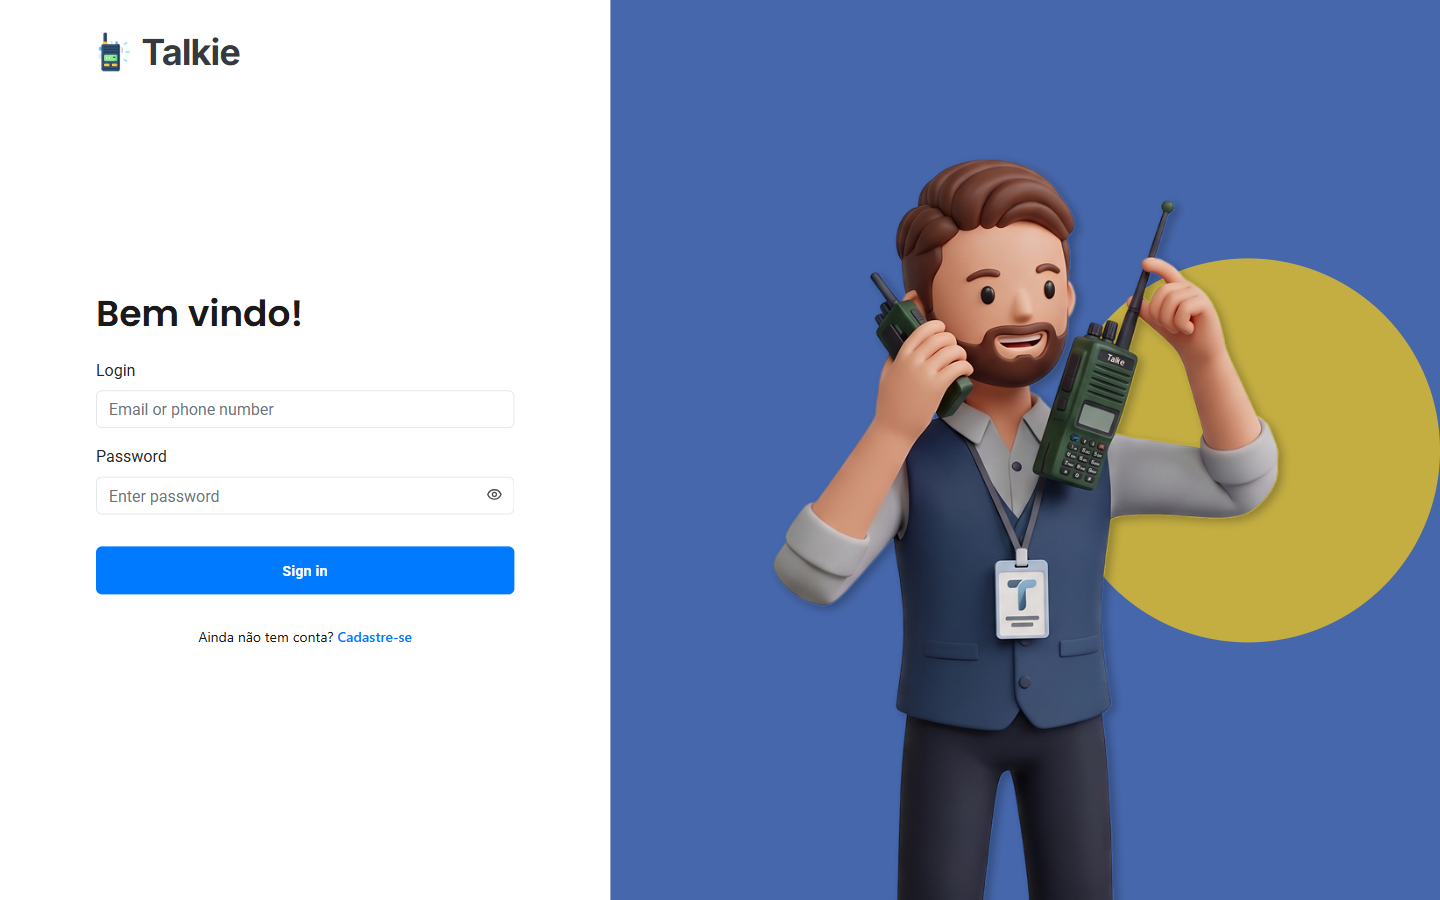
\includegraphics[width=\linewidth]{imagens/prints/01-login.png}
    \caption{Tela de login}
    \vspace{0.2cm}
    \small Fonte: elaboração própria (2026).
    \label{fig:impl-login}
\end{figure}

O \textit{layout} da tela divide a área em duas partes: o formulário à esquerda e uma ilustração à direita, composição também adotada na tela de cadastro. O formulário é controlado pela biblioteca React Hook Form, e a validação do preenchimento é feita por um esquema da biblioteca Zod, que indica o erro junto ao campo quando o e-mail está vazio ou malformado, antes de qualquer requisição à API. Se as credenciais forem recusadas, a mensagem devolvida pelo \textit{back-end} é exibida em um alerta acima do formulário.

Em caso de sucesso, a API devolve o token JWT, que o \textit{front-end} guarda no \textit{localStorage} do navegador e decodifica para obter o e-mail e o perfil do usuário. A partir daí, um interceptador da instância de requisições anexa o token a todas as chamadas à API. As rotas do sistema são envolvidas por um componente de proteção, que redireciona para o login quem não possui sessão válida e, nas rotas administrativas, devolve à página inicial quem não possui o perfil de administrador. Ao abrir a tela de login, qualquer sessão anterior é encerrada.

\subsubsection{Tela de Cadastro}
O cadastro permite que um visitante crie sua conta informando nome, CPF, e-mail e senha, com confirmação da senha. A conta é criada com o perfil de usuário comum e, ao final, o visitante é direcionado ao login, onde um alerta informa que a conta foi criada. A Figura~\ref{fig:impl-cadastro} apresenta o formulário e a Figura~\ref{fig:impl-cadastro-erros}, o mesmo formulário com dados inválidos.

\begin{figure}[H]
    \centering
    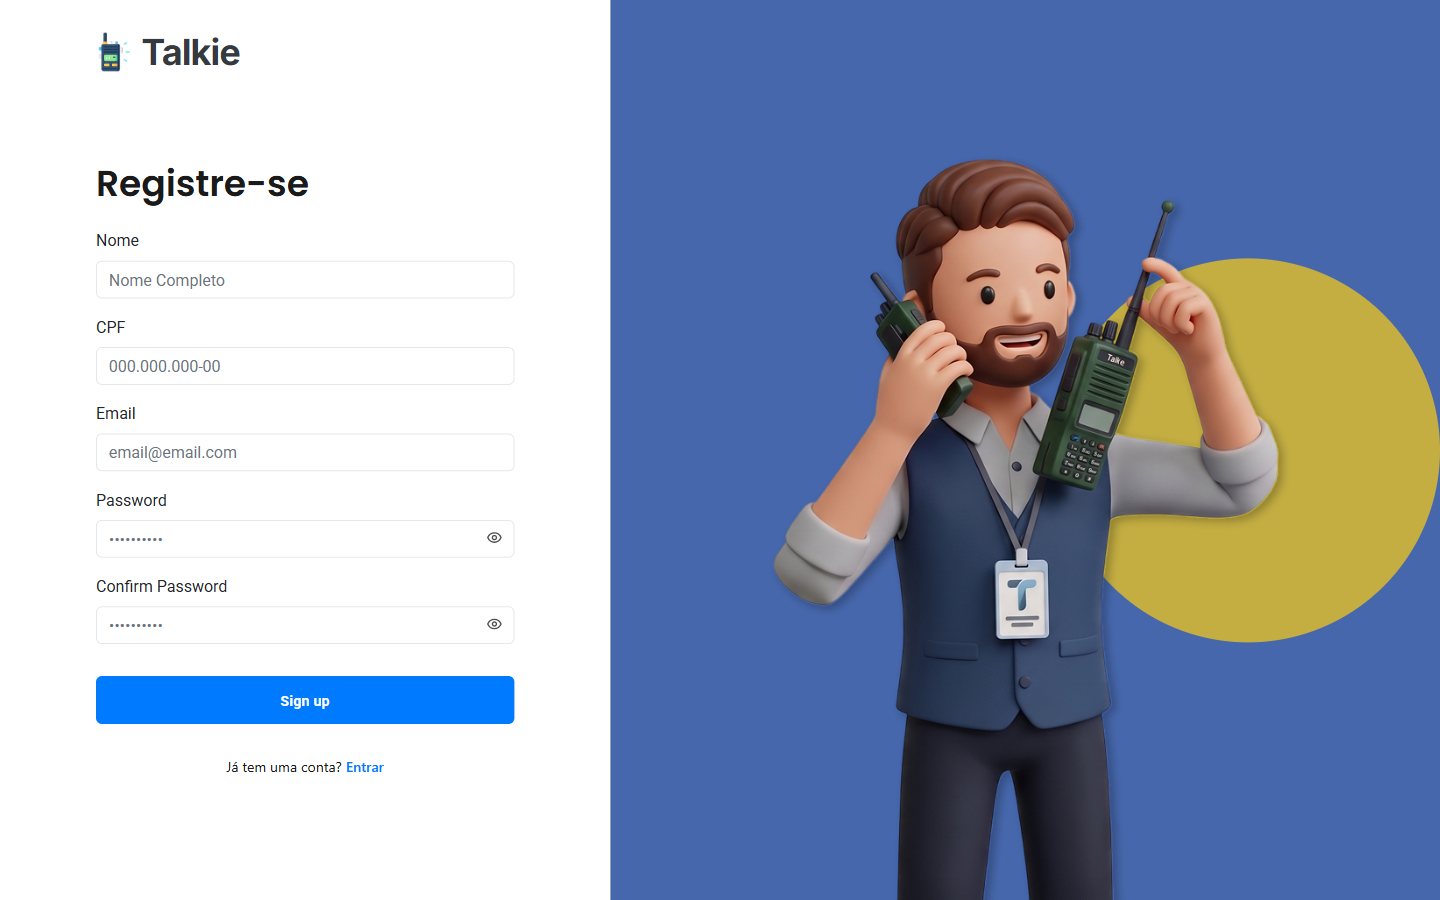
\includegraphics[width=\linewidth]{imagens/prints/02-cadastro.png}
    \caption{Tela de cadastro}
    \vspace{0.2cm}
    \small Fonte: elaboração própria (2026).
    \label{fig:impl-cadastro}
\end{figure}

\begin{figure}[H]
    \centering
    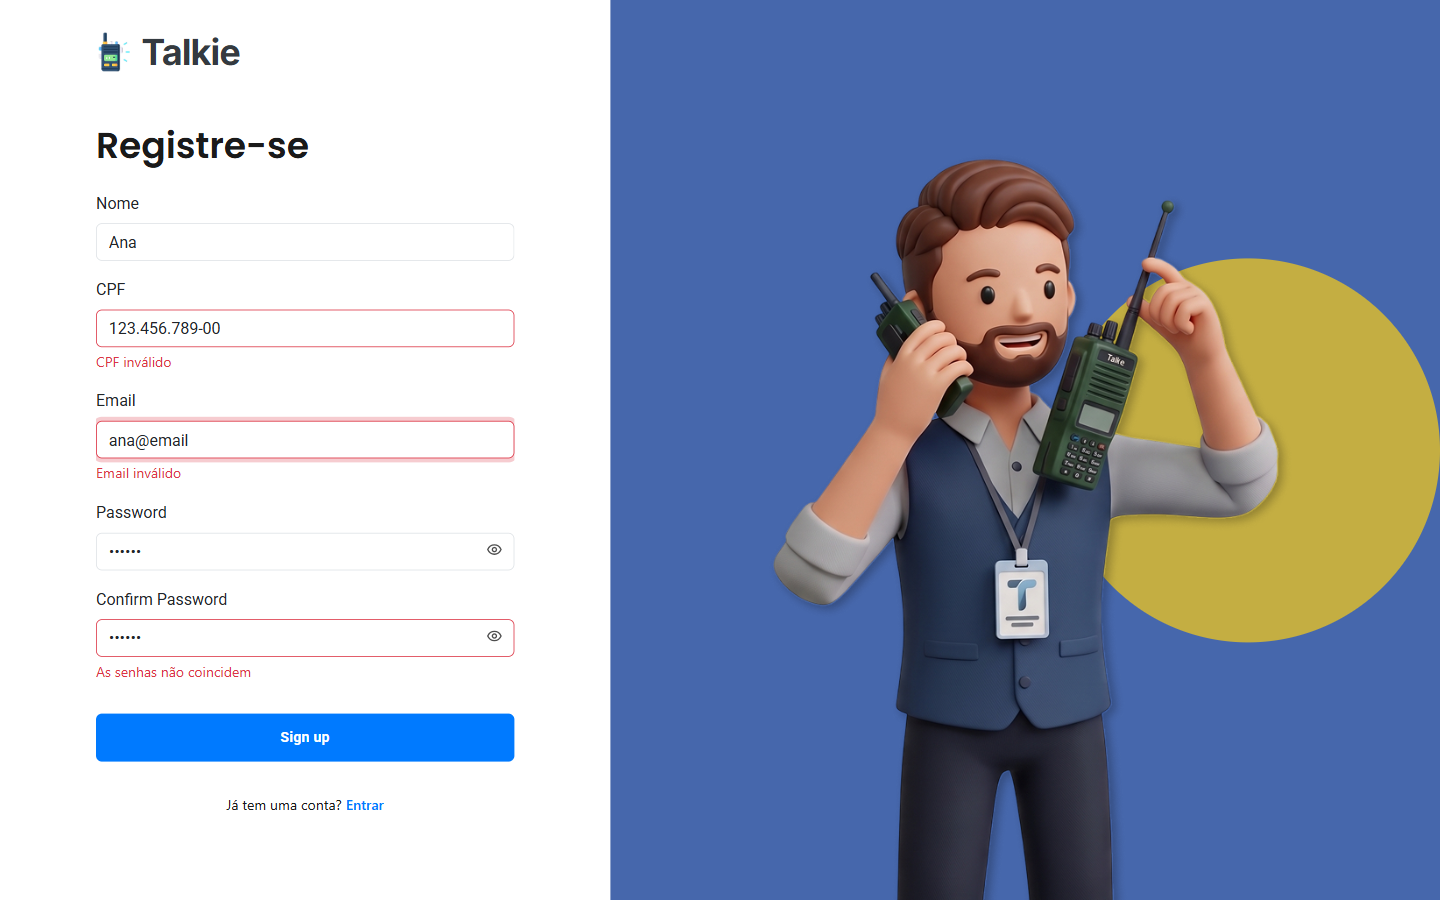
\includegraphics[width=\linewidth]{imagens/prints/03-cadastro-validacao.png}
    \caption{Tela de cadastro com mensagens de validação}
    \vspace{0.2cm}
    \small Fonte: elaboração própria (2026).
    \label{fig:impl-cadastro-erros}
\end{figure}

O formulário valida os dados no navegador, com mensagens em português exibidas junto a cada campo: o nome deve ter ao menos três caracteres, o e-mail deve ser válido, a senha deve ter ao menos seis caracteres e a confirmação deve ser igual à senha. O campo de CPF recebe uma máscara que formata o número enquanto ele é digitado, e sua validade é verificada por meio dos dígitos verificadores, e não apenas pela quantidade de caracteres. O campo de confirmação existe somente no \textit{front-end}: ele é removido antes do envio, e a API recebe apenas os demais dados.

Quando o CPF ou o e-mail informados já estão cadastrados, o \textit{back-end} recusa a requisição, e o \textit{front-end} associa a mensagem recebida ao campo correspondente, em vez de exibi-la como um erro genérico, o que indica ao usuário qual dado corrigir.

\subsubsection{Tela de Listagem de Ocorrências}
A página inicial do sistema, chamada de Geral, lista as ocorrências do usuário e resume sua situação. Para o usuário comum, a página se intitula ``Minhas Ocorrências'' e exibe as ocorrências que ele registrou, como mostra a Figura~\ref{fig:impl-lista-usuario}. Para o administrador, intitula-se ``Todas as Ocorrências'' e exibe todas as registradas, como mostra a Figura~\ref{fig:impl-lista-admin}.

\begin{figure}[H]
    \centering
    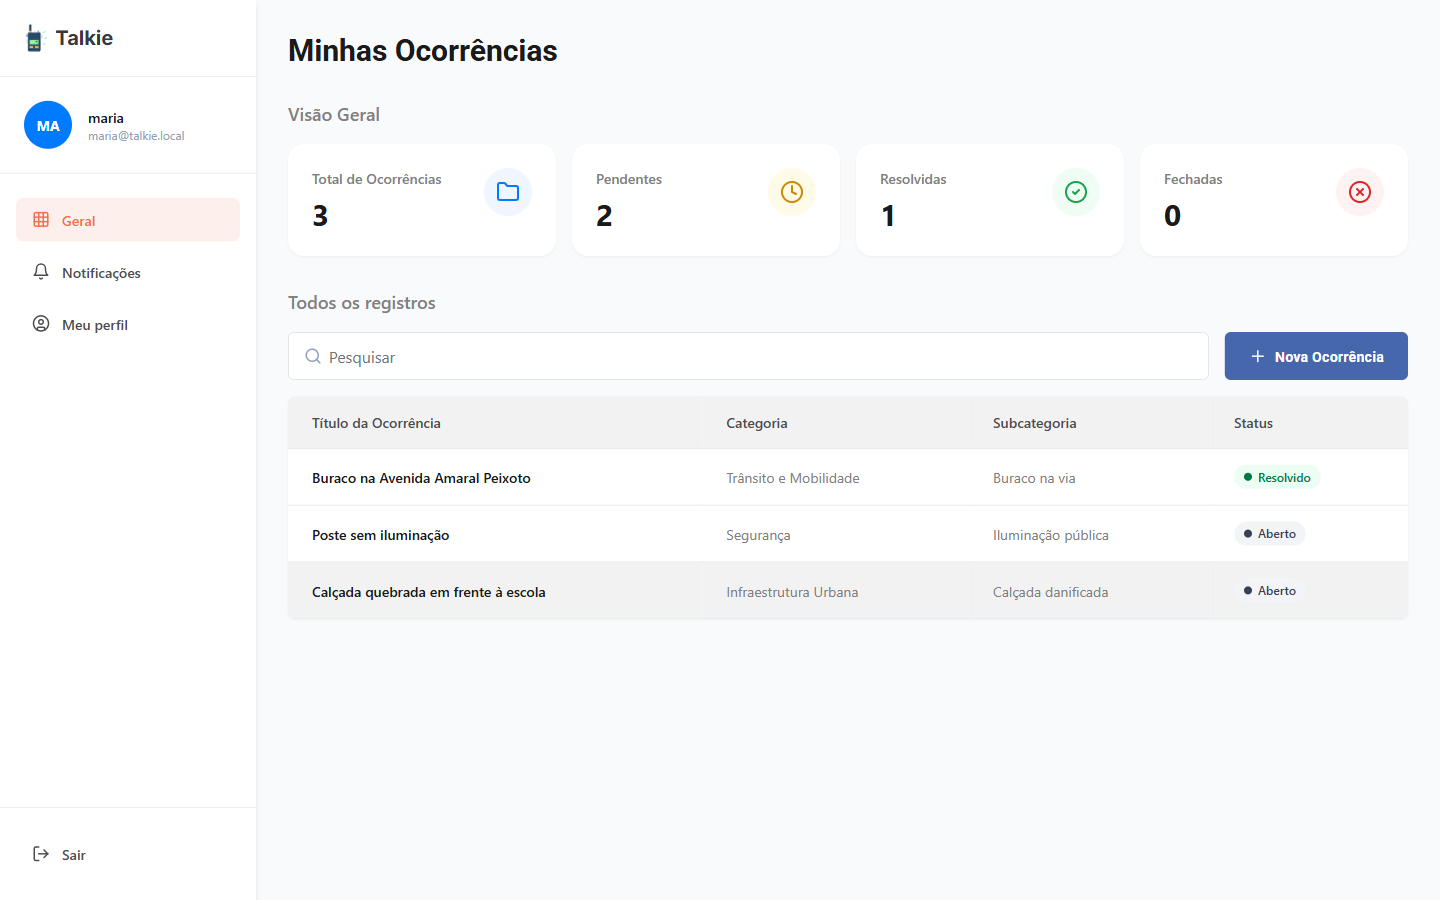
\includegraphics[width=\linewidth]{imagens/prints/04-listagem-ocorrencias-usuario.png}
    \caption{Listagem de ocorrências do usuário}
    \vspace{0.2cm}
    \small Fonte: elaboração própria (2026).
    \label{fig:impl-lista-usuario}
\end{figure}

\begin{figure}[H]
    \centering
    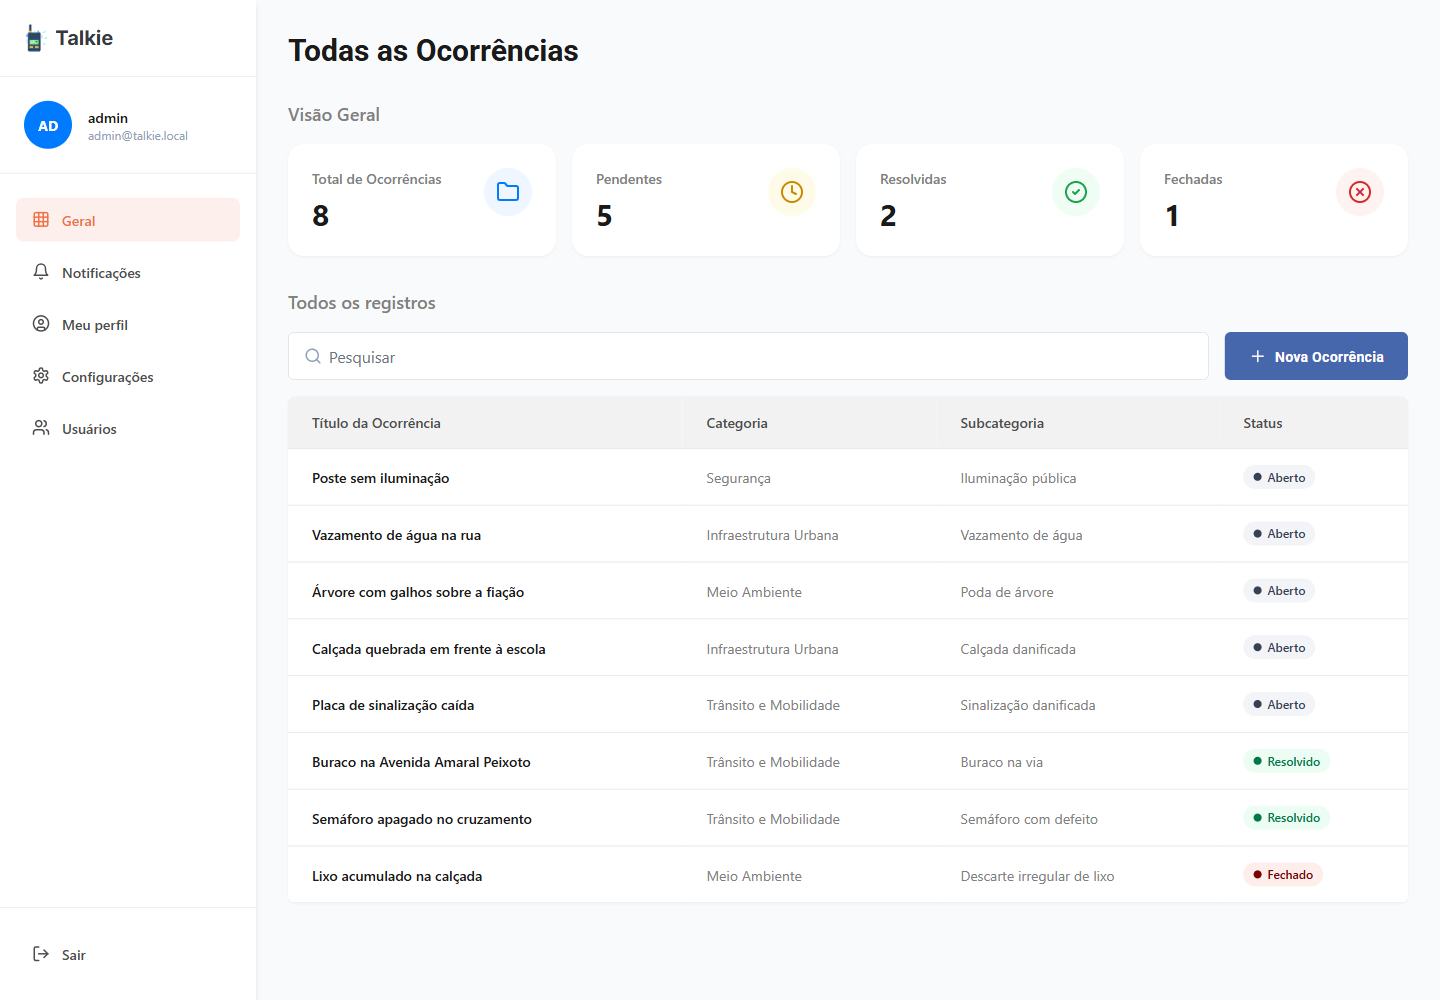
\includegraphics[width=\linewidth]{imagens/prints/06-listagem-ocorrencias-admin.png}
    \caption{Listagem de ocorrências do administrador}
    \vspace{0.2cm}
    \small Fonte: elaboração própria (2026).
    \label{fig:impl-lista-admin}
\end{figure}

A mesma página atende aos dois perfis. O componente é o mesmo, e a diferença está na origem dos dados e no comportamento da tabela: somente para o administrador as linhas são clicáveis e levam à tela de detalhes da ocorrência. Na parte superior, quatro cartões de resumo informam o total de ocorrências e as quantidades de pendentes, resolvidas e fechadas, o que dá uma visão geral antes da consulta à tabela.

A tabela apresenta título, categoria, subcategoria e situação de cada ocorrência. A situação é exibida em um selo colorido, com uma cor para cada status (aberto, resolvido e fechado), definida como \textit{token} no Tailwind CSS, o que mantém o mesmo código de cores em todas as telas em que o status aparece. O campo de pesquisa filtra a lista pelo título ou pelo nome da categoria, e o botão ``Nova Ocorrência'' leva ao formulário de registro.

\subsubsection{Tela de Criação de Ocorrência}
Nesta tela, o usuário registra uma nova ocorrência. O formulário reúne os dados de classificação, a localização, uma foto opcional e a descrição do problema, como mostra a Figura~\ref{fig:impl-criar}.

\begin{figure}[H]
    \centering
    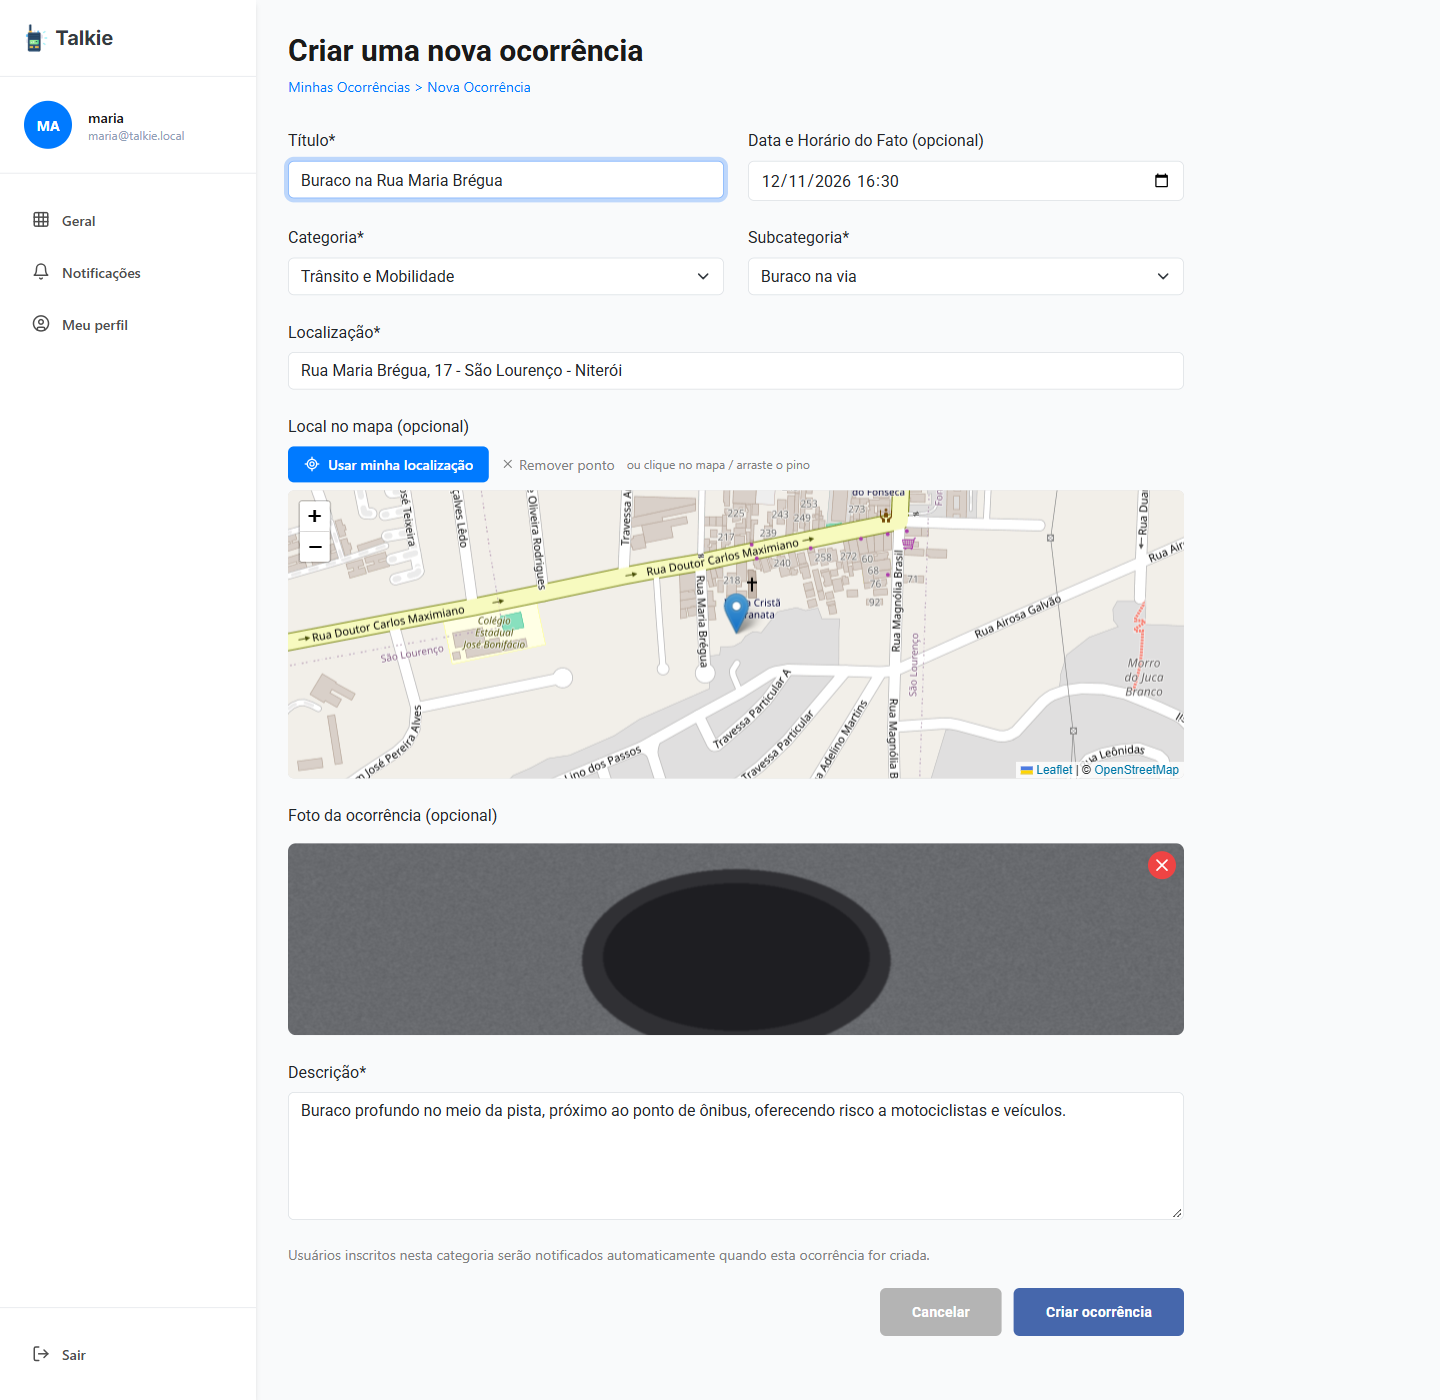
\includegraphics[width=\linewidth]{imagens/prints/05-nova-ocorrencia.png}
    \caption{Tela de criação de ocorrência}
    \vspace{0.2cm}
    \small Fonte: elaboração própria (2026).
    \label{fig:impl-criar}
\end{figure}

A classificação é feita em duas etapas encadeadas. O campo de subcategoria permanece desabilitado até que uma categoria seja escolhida e lista apenas as subcategorias da categoria selecionada, filtradas pelo identificador da categoria. Se o usuário troca de categoria, a subcategoria escolhida é descartada. Somente categorias e subcategorias ativas são oferecidas. O campo de data e horário do fato é opcional, e o esquema de validação rejeita datas futuras.

A localização combina três formas de preenchimento. O usuário pode digitar o endereço, clicar no mapa ou usar a posição do dispositivo, pelo botão ``Usar minha localização''. O mapa é exibido pela biblioteca Leaflet, com imagens do OpenStreetMap, e o pino pode ser arrastado para ajuste fino ou removido. Ao marcar um ponto, o sistema registra a latitude e a longitude e consulta o serviço Nominatim, que devolve um endereço sugerido para preencher o campo de localização. Se o usuário já tiver digitado o endereço, ele não é sobrescrito. Quando a posição vem do dispositivo, a precisão aproximada é informada, e uma precisão pior que 100 metros acompanha a recomendação de conferir o pino no mapa. A latitude e a longitude são validadas em conjunto, de modo que não é possível enviar apenas uma delas.

A imagem é opcional e aceita arquivos JPEG, PNG ou WebP de até 5 MB, com pré-visualização e possibilidade de remoção antes do envio. A imagem trafega em uma requisição separada, posterior à criação da ocorrência. Assim, uma falha no envio do arquivo não impede o registro dos dados. No \textit{back-end}, o tamanho é conferido, e o tipo do arquivo é identificado pela sua assinatura (os primeiros \textit{bytes}), e não pela extensão informada.

Ao final, o texto abaixo da descrição lembra o usuário de que os inscritos na categoria serão notificados. De fato, o registro da ocorrência dispara um evento que faz o \textit{back-end} enviar um e-mail aos usuários que assinam a categoria, mecanismo descrito na Subseção~\ref{sec:impl-notificacoes}.

\subsubsection{Tela de Detalhes da Ocorrência}
A tela de detalhes, restrita ao administrador, reúne as informações de uma ocorrência, o histórico de seus status e as ações para tratá-la. Ela é acessada pela listagem e está representada na Figura~\ref{fig:impl-detalhes}.

\begin{figure}[H]
    \centering
    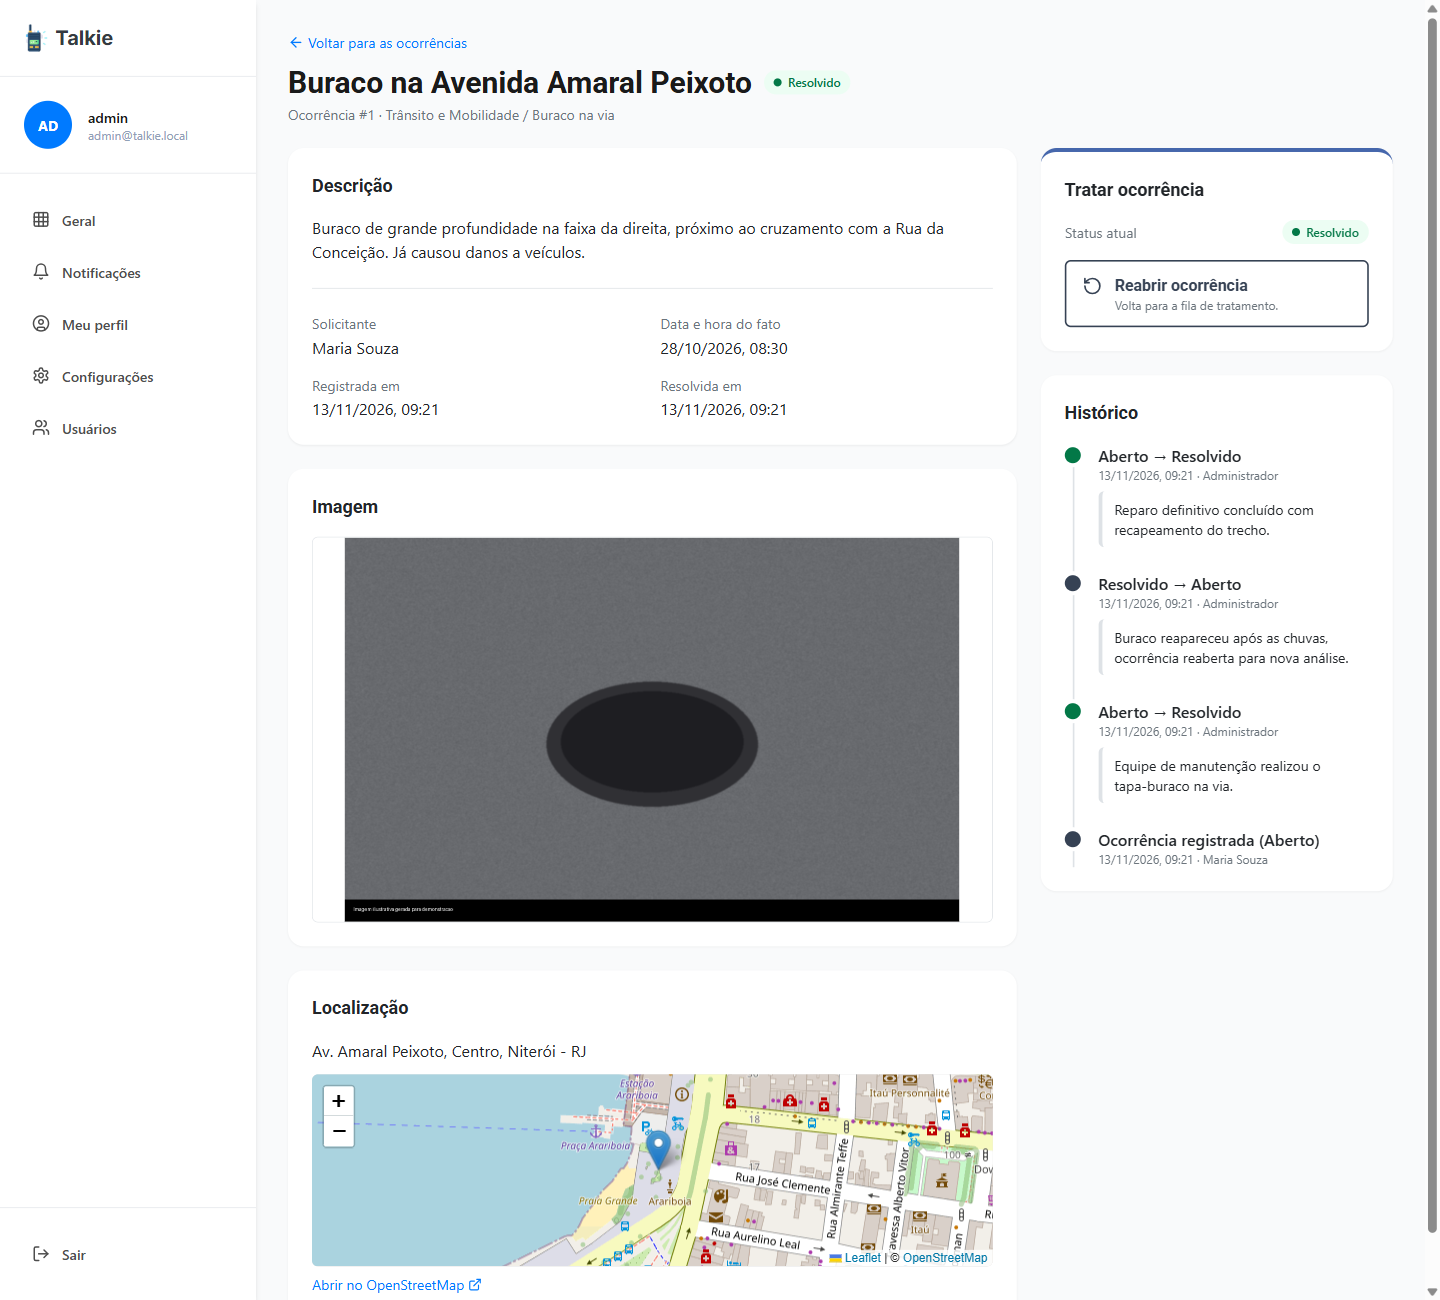
\includegraphics[width=\linewidth]{imagens/prints/07-detalhes-ocorrencia.png}
    \caption{Tela de detalhes de uma ocorrência já tratada}
    \vspace{0.2cm}
    \small Fonte: elaboração própria (2026).
    \label{fig:impl-detalhes}
\end{figure}

O \textit{layout} é dividido em duas colunas. A coluna principal apresenta o que foi reportado: a descrição, o solicitante, a data e hora do fato, a data de registro e a de resolução, a imagem e a localização. A imagem é baixada pelo \textit{front-end} como um arquivo binário e exibida a partir dele, porque o endereço da imagem exige o token JWT e, por isso, não pode ser carregado diretamente por uma \textit{tag} de imagem comum. Na localização, o mesmo componente de mapa da tela de criação é reutilizado em modo somente leitura, acompanhado de um \textit{link} para abrir o ponto no OpenStreetMap. Se o solicitante não marcou o ponto, uma mensagem informa a ausência. Quando o solicitante teve a conta excluída, o nome é substituído por ``Usuário excluído''.

A coluna lateral concentra o tratamento. O painel ``Tratar ocorrência'' mostra o status atual e as ações possíveis a partir dele: para uma ocorrência aberta, marcar como resolvida ou encerrar sem resolução, e, para uma ocorrência resolvida ou fechada, reabri-la. Cada ação tem uma cor própria, para que resolver e encerrar não sejam confundidas. A Figura~\ref{fig:impl-status} mostra a etapa seguinte à escolha de uma ação, em que o sistema solicita a confirmação e oferece um campo opcional para o motivo, de até 1000 caracteres, registrado no histórico. Se a alteração falha, o painel mantém a ação e o motivo informados, e o administrador pode tentar novamente.

\begin{figure}[H]
    \centering
    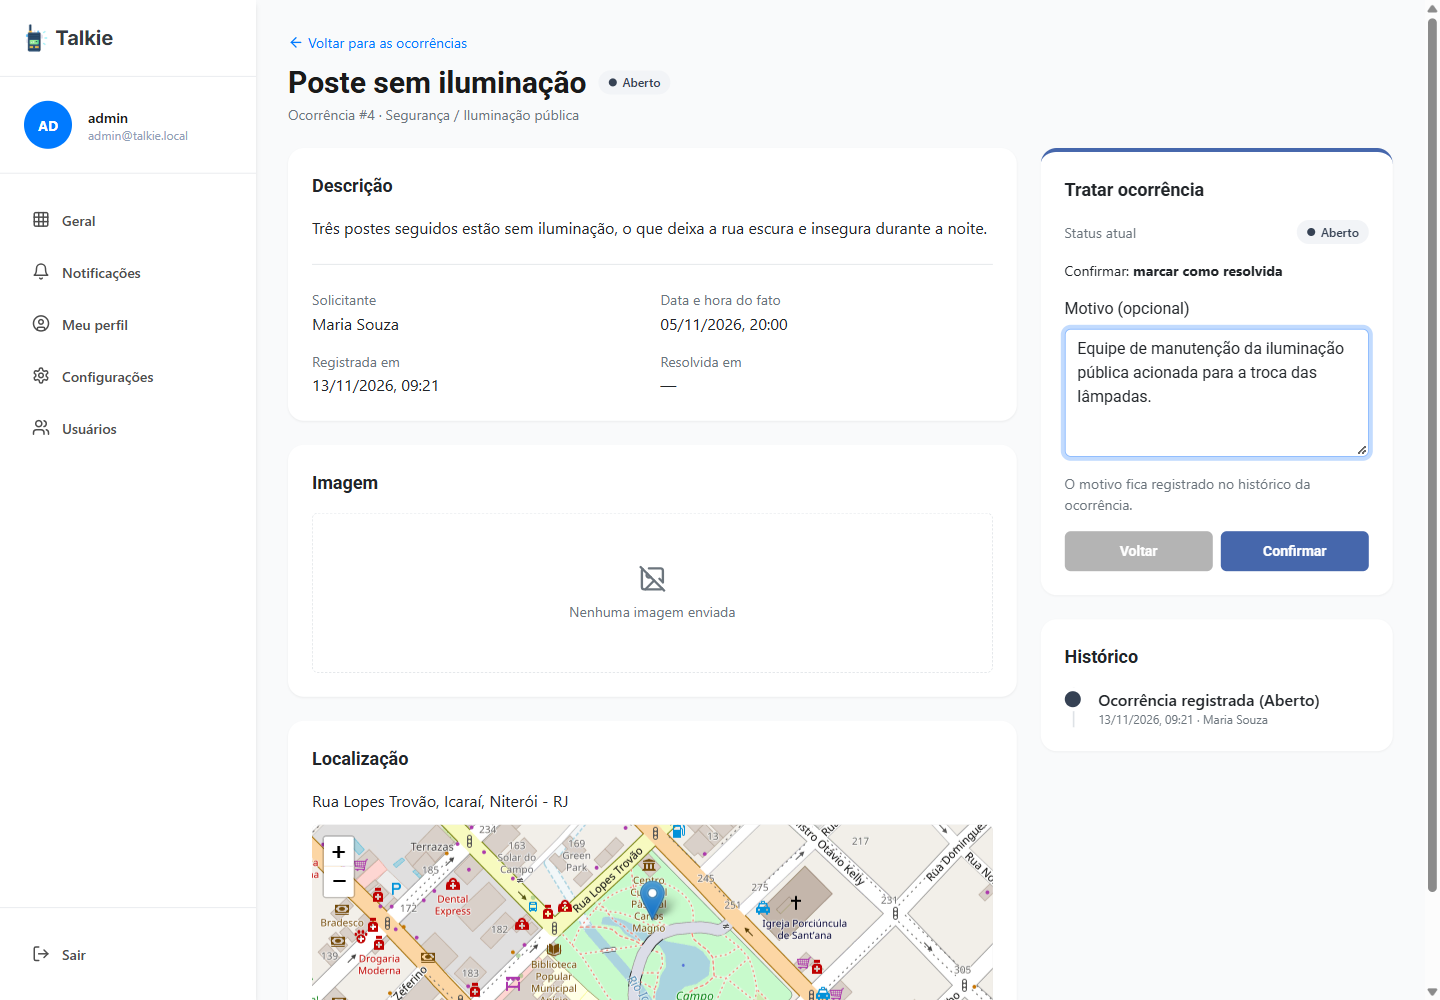
\includegraphics[width=\linewidth]{imagens/prints/09-alteracao-status.png}
    \caption{Confirmação da mudança de status, com motivo}
    \vspace{0.2cm}
    \small Fonte: elaboração própria (2026).
    \label{fig:impl-status}
\end{figure}

O histórico é exibido como uma linha do tempo, do evento mais recente para o mais antigo. Cada evento mostra a transição de status, a data, o autor e, quando existe, o motivo, em um bloco de citação, e o marcador recebe a cor do novo status. O primeiro evento de qualquer ocorrência é o de seu registro. Após cada mudança de status, a tela recarrega o histórico, de modo que a alteração apareça imediatamente. A Figura~\ref{fig:impl-detalhes} mostra uma ocorrência resolvida, reaberta e novamente resolvida, e cada passagem fica registrada com seu motivo.

\subsubsection{Tela de Categorias e Subcategorias}
As categorias e as subcategorias que classificam as ocorrências são gerenciadas pelo administrador na área de Configurações. A tela principal lista as categorias em uma tabela e, ao clicar em uma linha, expande as subcategorias correspondentes, como mostra a Figura~\ref{fig:impl-categorias}.

\begin{figure}[H]
    \centering
    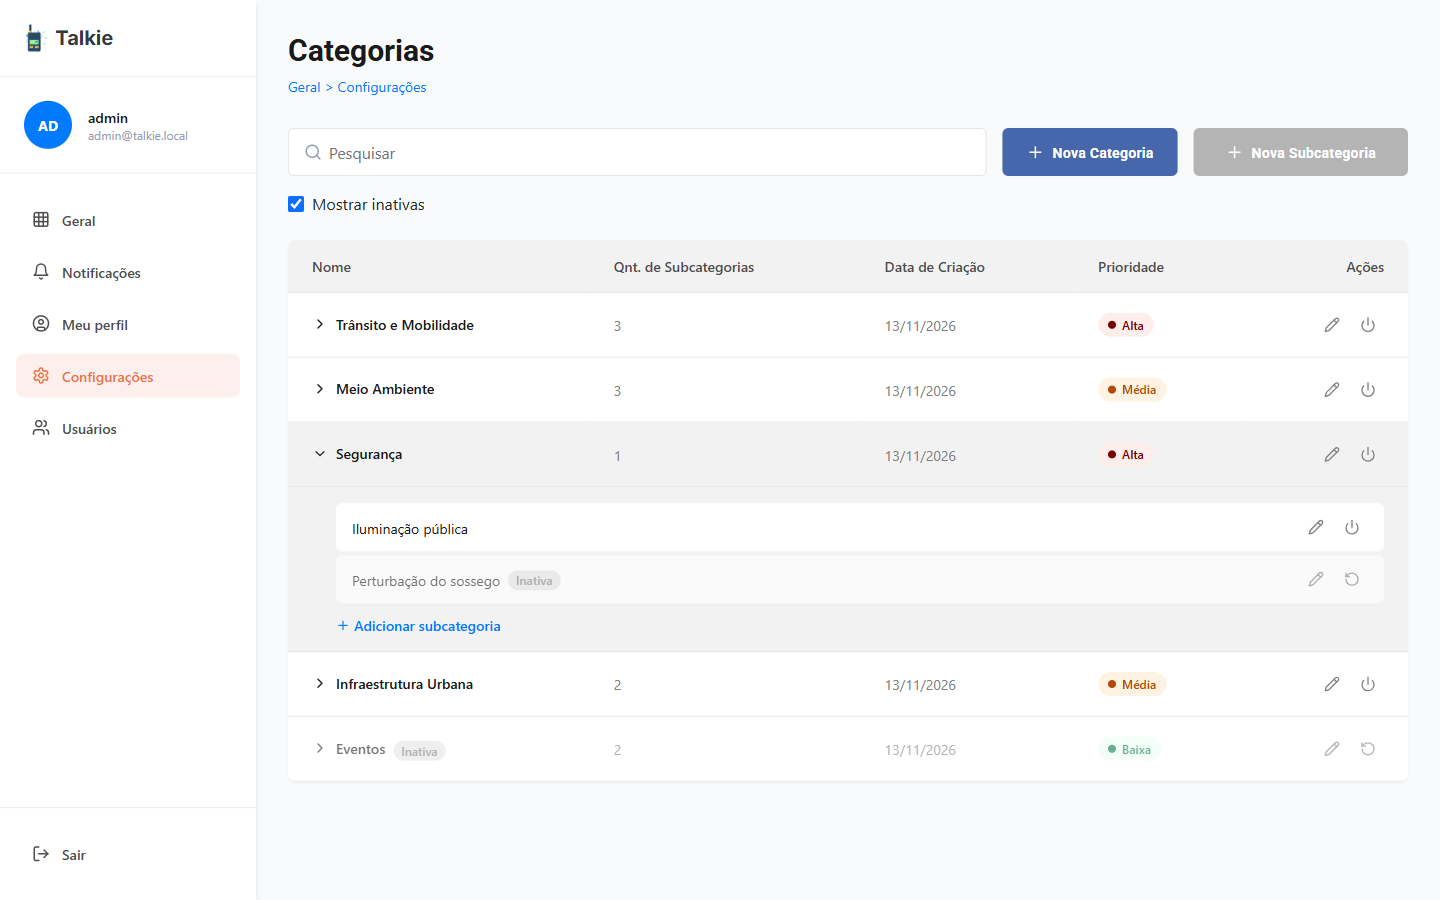
\includegraphics[width=\linewidth]{imagens/prints/15-categorias-inativas.png}
    \caption{Tela de categorias, com itens inativos e uma categoria expandida}
    \vspace{0.2cm}
    \small Fonte: elaboração própria (2026).
    \label{fig:impl-categorias}
\end{figure}

A tabela exibe o nome, a quantidade de subcategorias ativas, a data de criação e a prioridade de cada categoria, apresentada em um selo colorido (alta, média ou baixa). Cada linha oferece as ações de editar e desativar ou reativar, e o campo de pesquisa filtra as categorias pelo nome.

Categorias e subcategorias não são apagadas: a ação de desativar apenas as marca como inativas, o que as retira dos formulários de ocorrência e das assinaturas, mas preserva as ocorrências já registradas. Por padrão, a tela lista somente os itens ativos, e a opção ``Mostrar inativas'' inclui os demais, exibidos com aparência atenuada e um selo ``Inativa'', e acompanhados de um botão de reativação, como se vê na subcategoria ``Perturbação do sossego'' e na categoria ``Eventos''. Já os formulários de ocorrência e de assinatura consultam a API sem essa opção e recebem somente os itens ativos. Como a desativação altera o que os demais usuários enxergam, ela exige confirmação, por meio de uma janela que explica seus efeitos e informa que ela pode ser desfeita, apresentada na Figura~\ref{fig:impl-desativar}.

\begin{figure}[H]
    \centering
    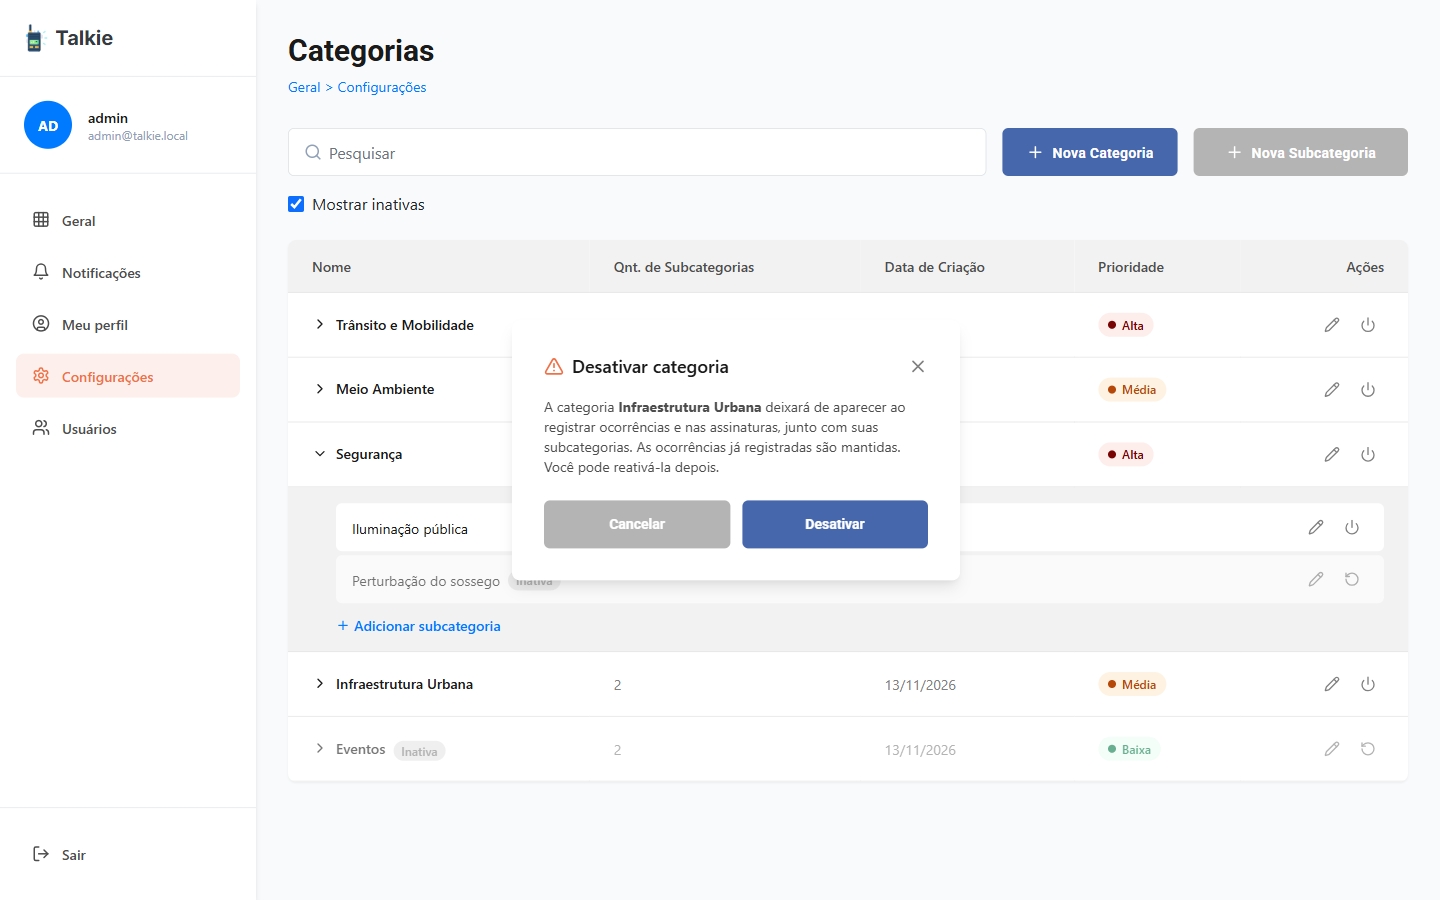
\includegraphics[width=\linewidth]{imagens/prints/16-categorias-desativar.png}
    \caption{Confirmação da desativação de uma categoria}
    \vspace{0.2cm}
    \small Fonte: elaboração própria (2026).
    \label{fig:impl-desativar}
\end{figure}

A criação e a edição usam formulários dedicados. A categoria é definida por nome, prioridade, ícone e cor, e os dois últimos são escolhidos em seletores visuais com opções predefinidas, em vez de campos de texto livre, como mostra a Figura~\ref{fig:impl-nova-categoria}. A subcategoria é definida por seu nome e pela categoria a que pertence, como mostra a Figura~\ref{fig:impl-nova-subcategoria}. Ao adicionar uma subcategoria a partir da linha expandida de uma categoria, esta já vem selecionada no formulário. Cada formulário é reaproveitado para a edição: quando a rota inclui o identificador do item, a mesma página carrega seus dados e atualiza o registro em vez de criar um novo.

\begin{figure}[H]
    \centering
    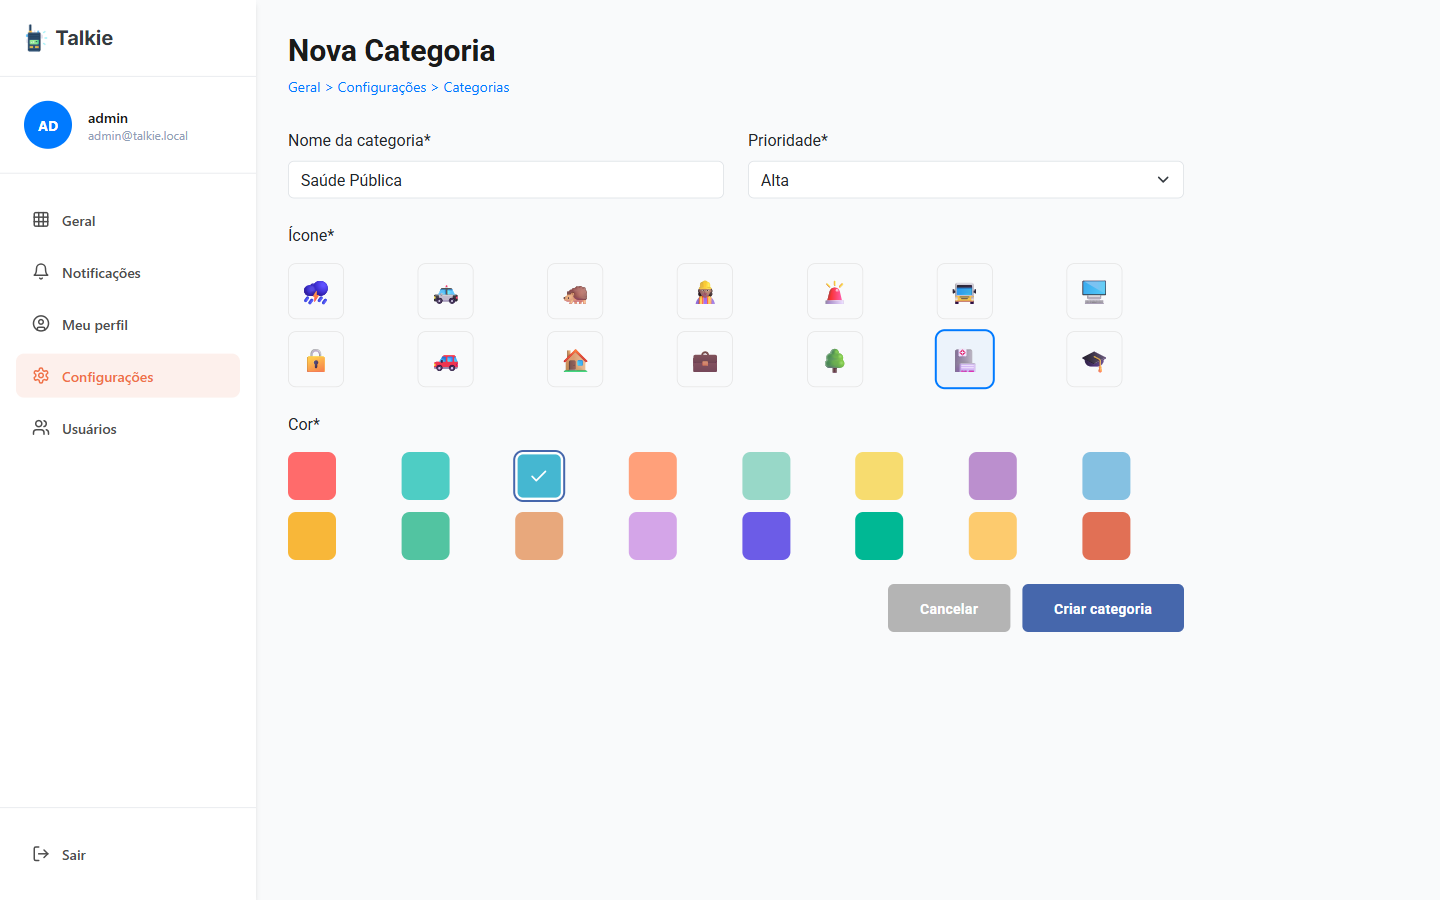
\includegraphics[width=\linewidth]{imagens/prints/17-nova-categoria.png}
    \caption{Formulário de criação de categoria}
    \vspace{0.2cm}
    \small Fonte: elaboração própria (2026).
    \label{fig:impl-nova-categoria}
\end{figure}

\begin{figure}[H]
    \centering
    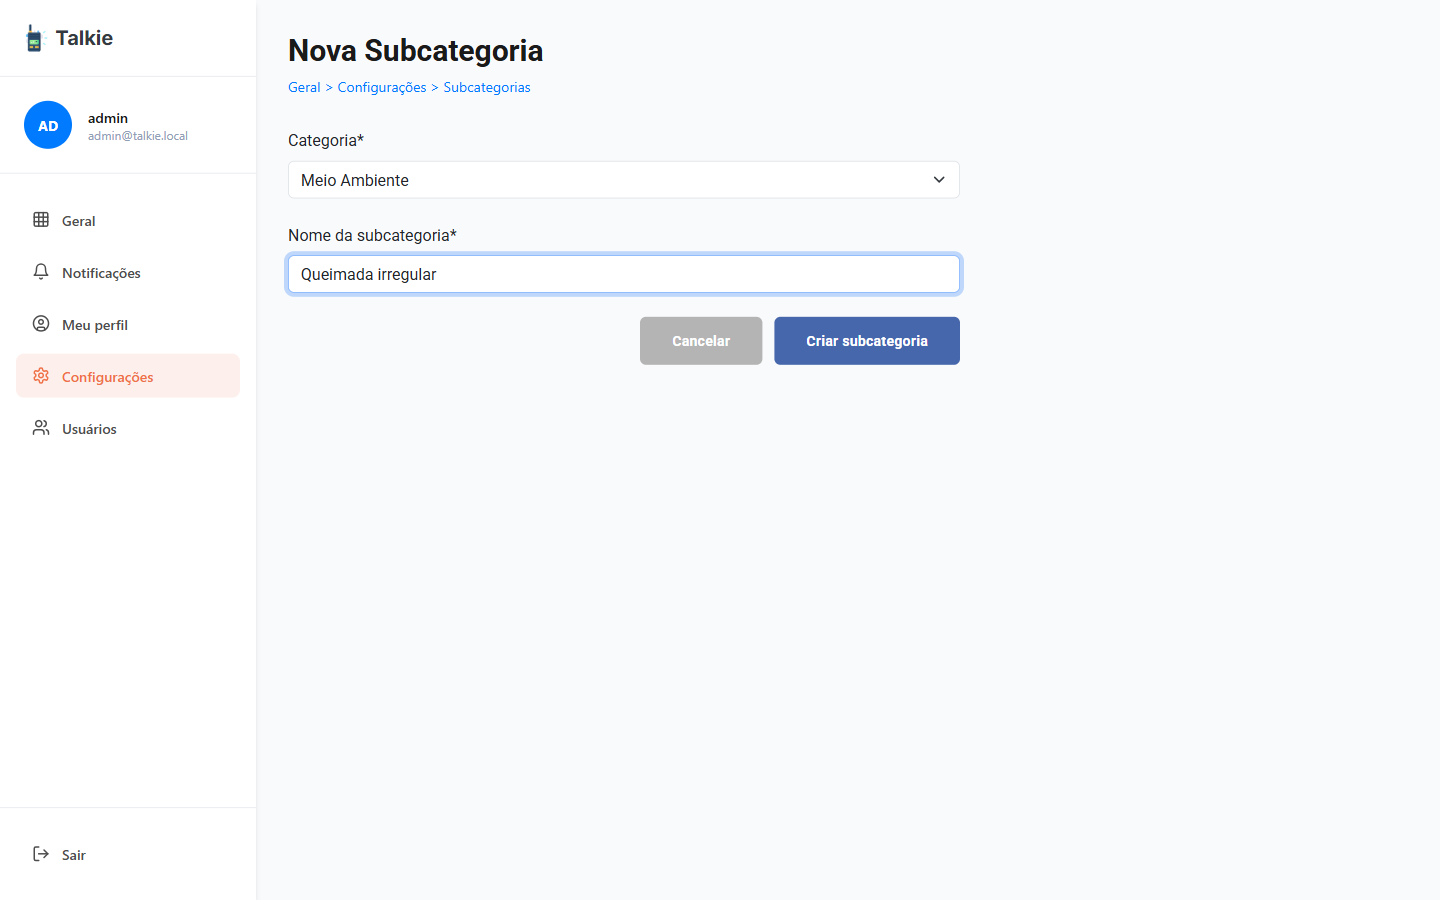
\includegraphics[width=\linewidth]{imagens/prints/18-nova-subcategoria.png}
    \caption{Formulário de criação de subcategoria}
    \vspace{0.2cm}
    \small Fonte: elaboração própria (2026).
    \label{fig:impl-nova-subcategoria}
\end{figure}

\subsubsection{Tela de Notificações e Assinaturas}
\label{sec:impl-notificacoes}
Na tela de Notificações, o usuário escolhe as categorias que deseja acompanhar e consulta as ocorrências delas. A parte superior lista suas assinaturas, e a inferior, a tabela ``Todas as Notificações'', como mostra a Figura~\ref{fig:impl-assinaturas}.

\begin{figure}[H]
    \centering
    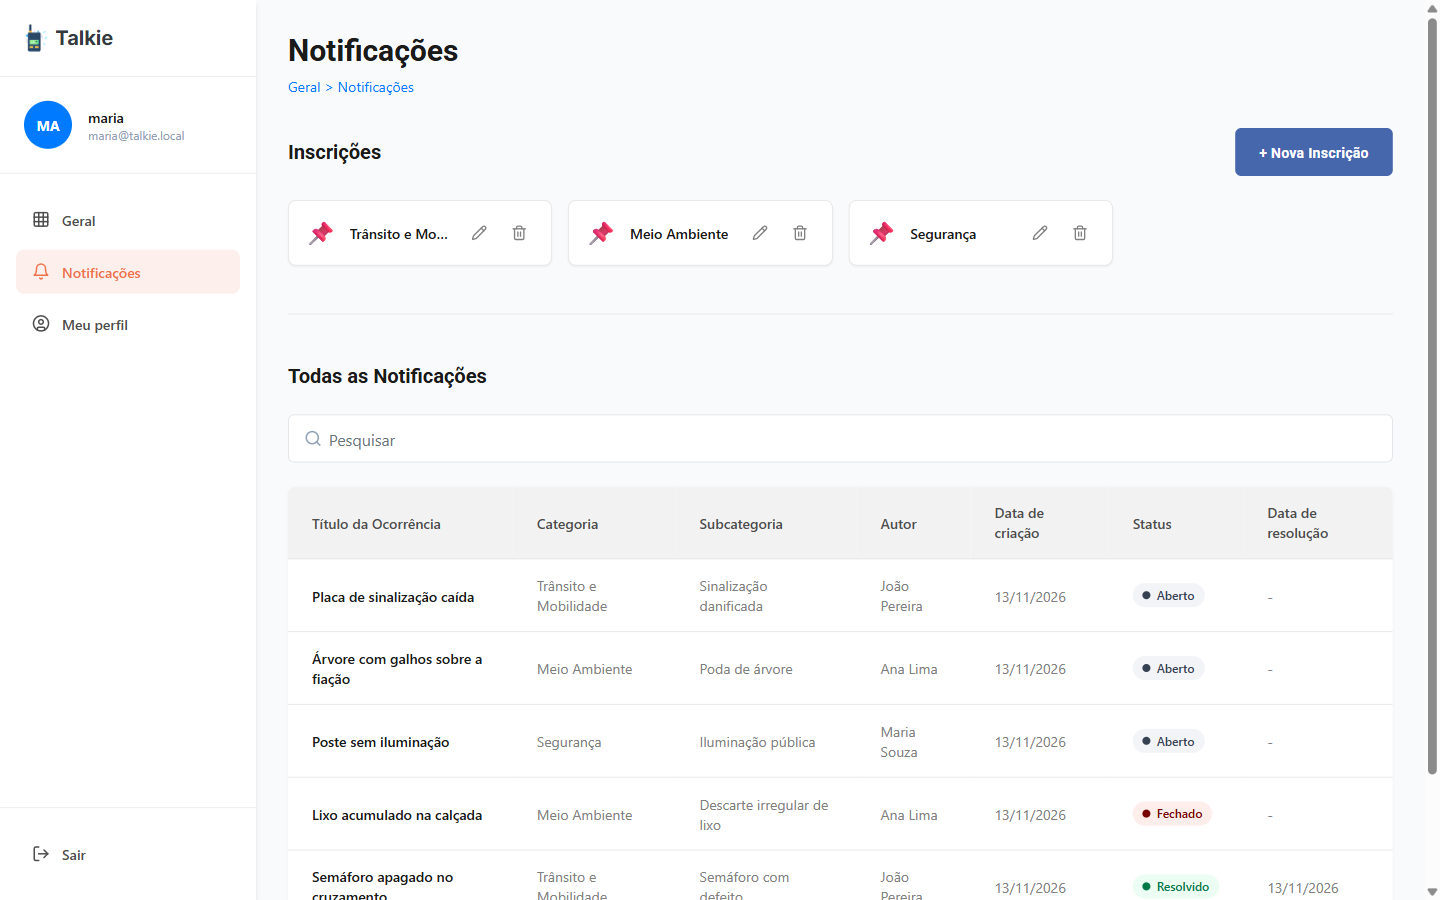
\includegraphics[width=\linewidth]{imagens/prints/10-assinaturas.png}
    \caption{Tela de notificações e assinaturas}
    \vspace{0.2cm}
    \small Fonte: elaboração própria (2026).
    \label{fig:impl-assinaturas}
\end{figure}

Cada assinatura é exibida em um cartão com o nome da categoria e dois botões, um para trocar a categoria e outro para cancelar a assinatura. O cancelamento solicita confirmação. A tabela abaixo reúne as ocorrências das categorias assinadas, com título, categoria, subcategoria, autor, datas e status, e pode ser pesquisada pelo título ou pela categoria.

A assinatura é feita pelo botão ``Nova Inscrição'', que abre a janela apresentada na Figura~\ref{fig:impl-nova-inscricao}. A lista de categorias oferecidas exclui as categorias inativas e aquelas em que o usuário já está inscrito, o que evita assinaturas repetidas; se todas já foram assinadas, a janela informa isso. A troca de categoria de uma assinatura existente é feita por duas chamadas à API, uma para cancelar a assinatura anterior e outra para criar a nova, e não por uma operação única de atualização.

\begin{figure}[H]
    \centering
    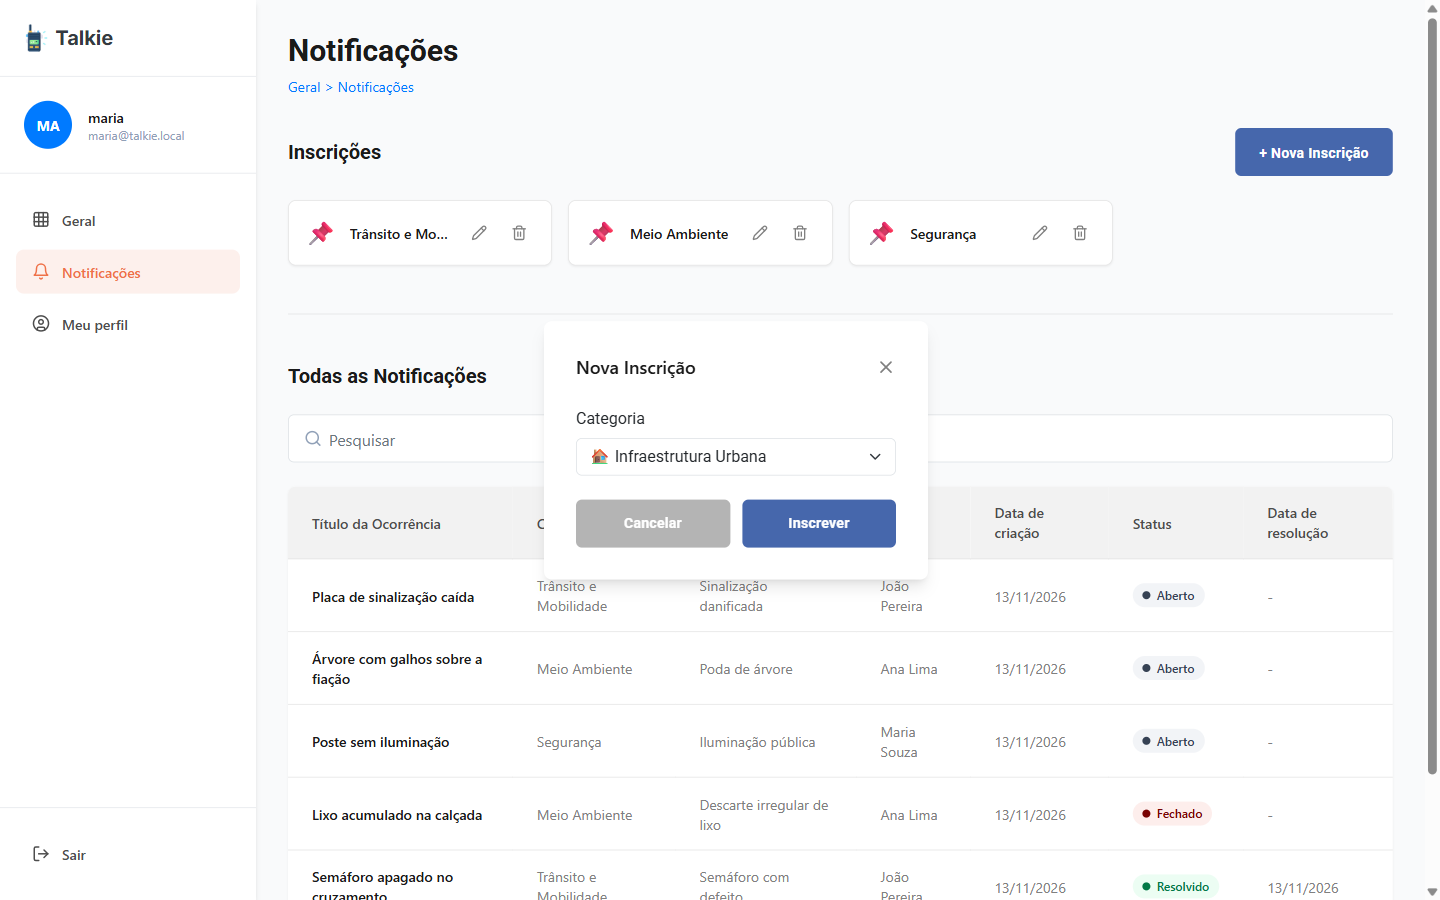
\includegraphics[width=\linewidth]{imagens/prints/11-assinaturas-nova-inscricao.png}
    \caption{Janela de nova inscrição em uma categoria}
    \vspace{0.2cm}
    \small Fonte: elaboração própria (2026).
    \label{fig:impl-nova-inscricao}
\end{figure}

As assinaturas também alimentam as notificações por e-mail. Quando uma ocorrência é registrada, o serviço de ocorrências publica um evento, que um \textit{listener} recebe e repassa ao serviço de e-mail, responsável por enviar uma mensagem a cada usuário que assina a categoria da ocorrência. Em ambiente de desenvolvimento, essas mensagens são capturadas pelo MailHog, servidor de e-mail de testes que permite conferi-las sem enviar mensagens reais.

\subsubsection{Tela de Usuários}
A tela de Usuários, restrita ao administrador, lista as contas cadastradas, como mostra a Figura~\ref{fig:impl-usuarios}. A tabela apresenta nome, e-mail, CPF, data de criação e permissão de cada usuário, esta última em um selo que distingue administradores de usuários comuns. O campo de pesquisa filtra a lista pelo nome ou pelo e-mail.

\begin{figure}[H]
    \centering
    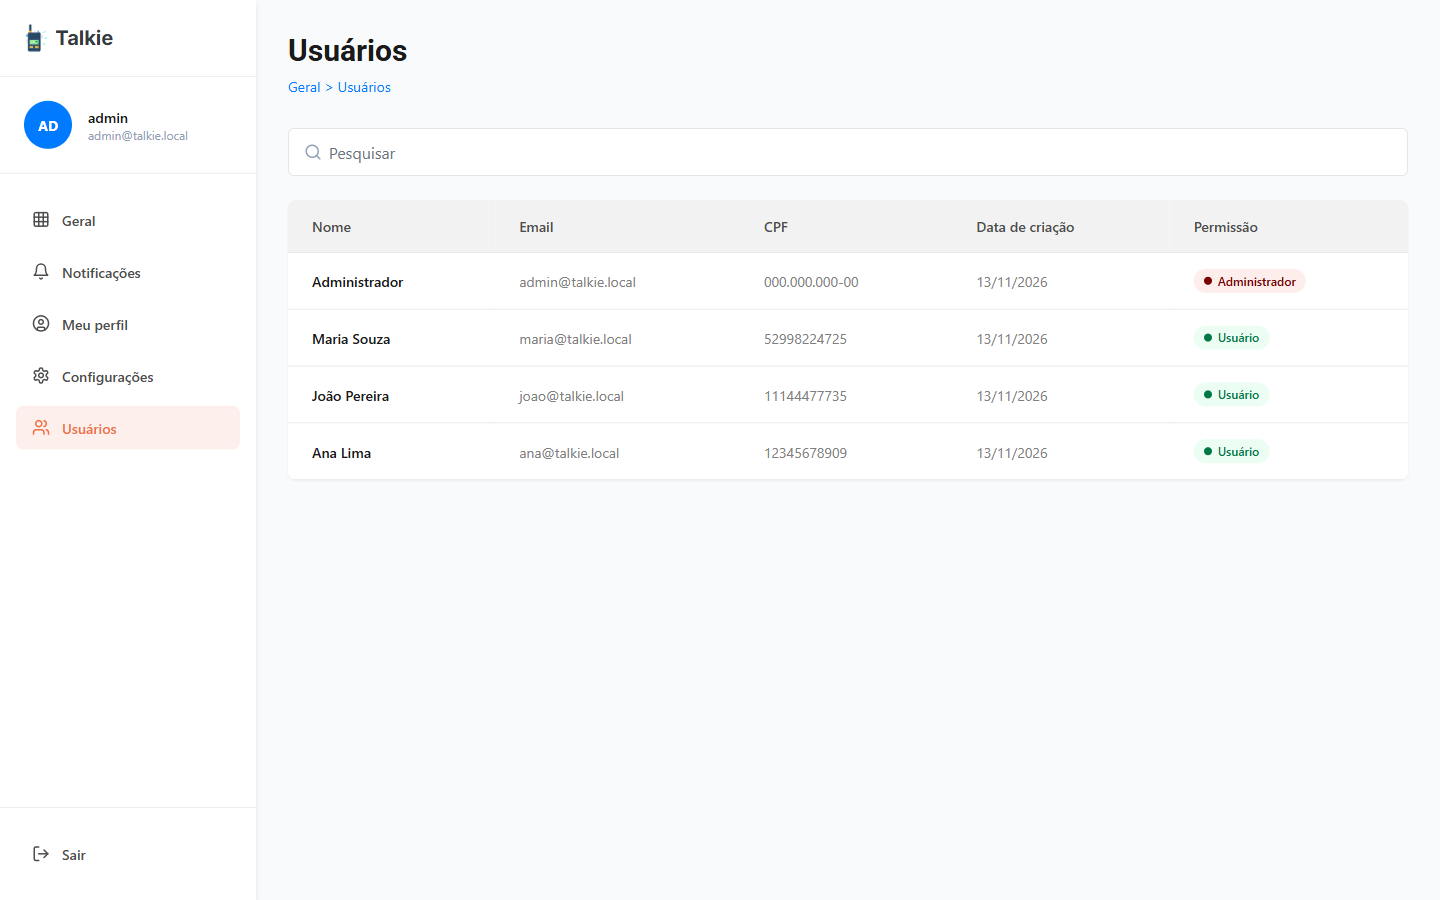
\includegraphics[width=\linewidth]{imagens/prints/19-usuarios.png}
    \caption{Tela de usuários}
    \vspace{0.2cm}
    \small Fonte: elaboração própria (2026).
    \label{fig:impl-usuarios}
\end{figure}

A tela é somente de consulta: não há ações de edição ou exclusão sobre as contas. O acesso a ela depende do perfil de administrador em dois níveis: o \textit{front-end} oculta o item do menu e bloqueia a rota, e o \textit{back-end} restringe a consulta de usuários por meio do Spring Security, de modo que o bloqueio não dependa apenas da interface. O mesmo vale para as demais operações administrativas, como a alteração de status, a consulta ao histórico e a criação, alteração e desativação de categorias e subcategorias.

\subsubsection{Tela de Meu Perfil e Exclusão de Conta}
A tela Meu perfil, disponível a todos os usuários, exibe o e-mail e o perfil da conta e permite excluí-la, como mostra a Figura~\ref{fig:impl-perfil}. A exclusão fica em uma seção separada, intitulada ``Zona de perigo'', destacada em vermelho, que descreve as consequências da ação antes de o usuário iniciá-la.

\begin{figure}[H]
    \centering
    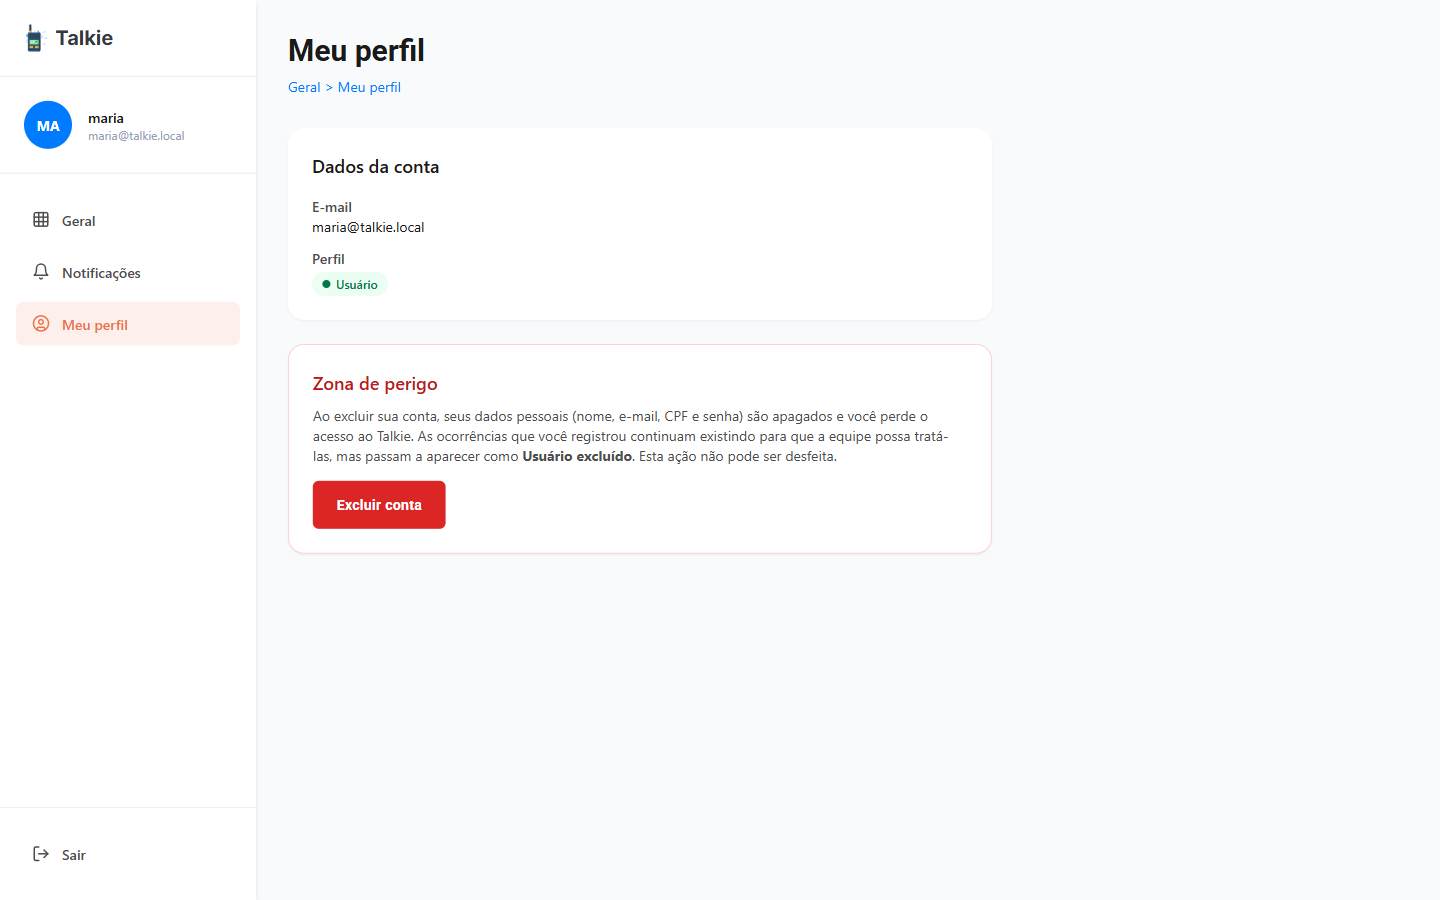
\includegraphics[width=\linewidth]{imagens/prints/12-perfil.png}
    \caption{Tela de perfil do usuário}
    \vspace{0.2cm}
    \small Fonte: elaboração própria (2026).
    \label{fig:impl-perfil}
\end{figure}

Por ser irreversível, a exclusão é confirmada em uma janela que exige a senha do usuário, como mostra a Figura~\ref{fig:impl-exclusao}. Ao confirmar, o \textit{front-end} envia a senha à API, que a confere antes de prosseguir. O identificador da conta a excluir é obtido do token, e não da requisição, de modo que um usuário só consegue excluir a própria conta. Em caso de sucesso, a sessão é encerrada e o usuário é redirecionado ao login.

\begin{figure}[H]
    \centering
    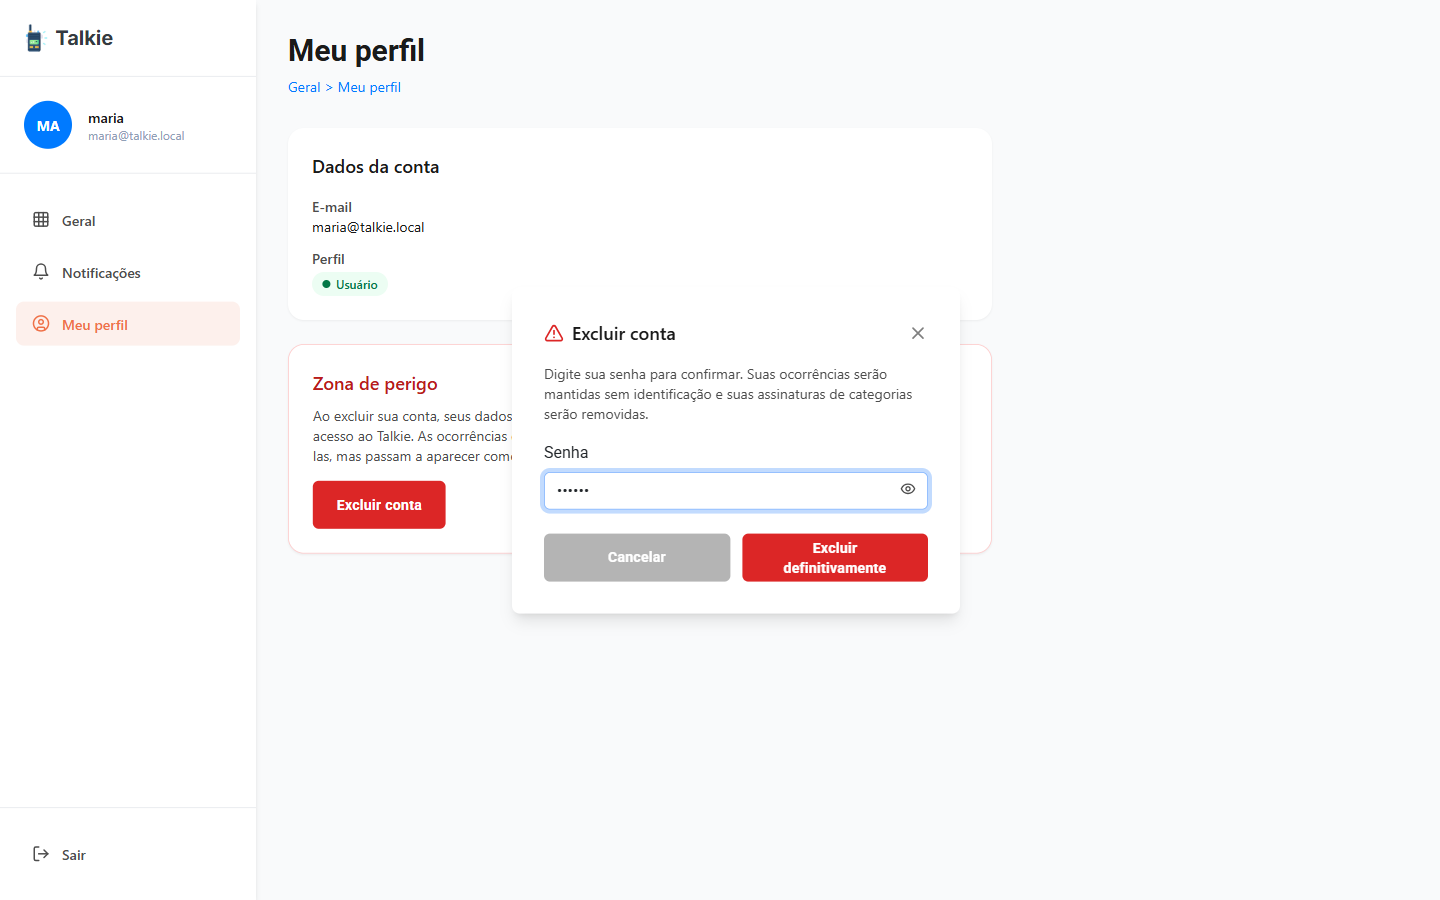
\includegraphics[width=\linewidth]{imagens/prints/13-exclusao-conta.png}
    \caption{Confirmação da exclusão de conta mediante senha}
    \vspace{0.2cm}
    \small Fonte: elaboração própria (2026).
    \label{fig:impl-exclusao}
\end{figure}

No \textit{back-end}, a exclusão anonimiza os dados em vez de apagar tudo. As ocorrências registradas pelo usuário, o histórico de status e as categorias que ele criou são mantidos, com a referência ao autor esvaziada, e o \textit{front-end} os exibe como ``Usuário excluído''. As assinaturas, que só têm utilidade para o próprio usuário, são removidas. Todas essas operações ocorrem em uma única transação, de modo que uma falha em qualquer etapa desfaz a exclusão inteira. O sistema também impede a exclusão do único administrador, para que a plataforma não fique sem quem a gerencie.

\subsection{Uso de Inteligência Artificial no Desenvolvimento}
O desenvolvimento do Talkie contou com o apoio de ferramentas de IA (Inteligência Artificial) em uma parte do projeto. O \textit{back-end} e o design das telas foram construídos manualmente. No \textit{front-end}, a IA foi utilizada principalmente na construção inicial do projeto, o chamado \textit{scaffold}, que reúne a estrutura-base de pastas, configurações e arquivos iniciais, e na criação dos componentes. O modelo utilizado foi o Claude, da Anthropic, com o MCP (\textit{Model Context Protocol}) do Figma instalado, recurso que permite à IA acessar os designs elaborados no Figma.

A experiência prévia com o \textit{framework} React permitiu avaliar o código gerado e corrigir os erros que surgiram ao longo do desenvolvimento. A IA foi empregada, portanto, com o objetivo de otimizar o início do trabalho, e não como substituta do conhecimento prévio sobre a tecnologia.


\section{Conclusão}
Nesta seção serão apresentadas as considerações finais, destacando as contribuições
esperadas do projeto, os resultados e os encaminhamentos para etapas futuras.


\begin{thebibliography}{99}

\bibitem{cor-rio}
PREFEITURA DO RIO DE JANEIRO.
\textit{Prefeitura lança COR.Rio, aplicativo que informa sobre ocorrências na cidade em tempo real}.
Prefeitura do Rio, [s.d.].
Disponível em: \url{https://l1nq.com/5menj}.
Acesso em: 16 dez. 2025.

\bibitem{waze}
WAZE.
\textit{Apps — Waze}.
Waze, 2025.
Disponível em: \url{https://www.waze.com/pt-BR/apps/}.
Acesso em: 16 dez. 2025.

\bibitem{1746}
CENTRAL 1746.
\textit{Portal Rio 1746}.
1746.rio, 2025.
Disponível em: \url{https://www.1746.rio/hc/pt-br}.
Acesso em: 16 dez. 2025.

\bibitem{duarte2014}
DUARTE, Pierre.
\textit{Aplicativos mapeiam problemas na cidade}.
JusBrasil, 11 maio 2014.
Disponível em: \url{https://www.jusbrasil.com.br/noticias/aplicativos-mapeiam-problemas-na-cidade/118684720}.
Acesso em: 16 dez. 2025.

\bibitem{sommerville}
SOMMERVILLE, Ian.
\textit{Engenharia de software}.
10. ed. São Paulo: Pearson Education do Brasil, 2018.

\end{thebibliography}


\end{document}
